% A LaTeX template for MSc Thesis submissions to 
% Politecnico di Milano (PoliMi) - School of Industrial and Information Engineering
%
% S. Bonetti, A. Gruttadauria, G. Mescolini, A. Zingaro
% e-mail: template-tesi-ingind@polimi.it
%
% Last Revision: October 2021
%
% Copyright 2021 Politecnico di Milano, Italy. NC-BY

\documentclass{Configuration_Files/PoliMi3i_thesis}

%------------------------------------------------------------------------------
%	REQUIRED PACKAGES AND  CONFIGURATIONS
%------------------------------------------------------------------------------

% CONFIGURATIONS

\usepackage{graphicx}

\usepackage{parskip} % For paragraph layout
\usepackage{setspace} % For using single or double spacing
\usepackage{emptypage} % To insert empty pages
\usepackage{multicol} % To write in multiple columns (executive summary)
\setlength\columnsep{15pt} % Column separation in executive summary
\setlength\parindent{0pt} % Indentation
\raggedbottom  

% PACKAGES FOR TITLES
\usepackage{titlesec}
% \titlespacing{\section}{left spacing}{before spacing}{after spacing}
\titlespacing{\section}{0pt}{3.3ex}{2ex}
\titlespacing{\subsection}{0pt}{3.3ex}{1.65ex}
\titlespacing{\subsubsection}{0pt}{3.3ex}{1ex}
\usepackage{color}

% PACKAGES FOR LANGUAGE AND FONT
\usepackage[english]{babel} % The document is in English  
\usepackage[utf8]{inputenc} % UTF8 encoding
\usepackage[T1]{fontenc} % Font encoding
\usepackage[11pt]{moresize} % Big fonts

% PACKAGES FOR IMAGES
\usepackage{graphicx}
\usepackage{transparent} % Enables transparent images
\usepackage{eso-pic} % For the background picture on the title page
\usepackage{subfig} % Numbered and caption subfigures using \subfloat.
\usepackage{tikz} % A package for high-quality hand-made figures.
\usetikzlibrary{}
\graphicspath{{./Images/}} % Directory of the images
\usepackage{caption} % Coloured captions
\usepackage{xcolor} % Coloured captions
\usepackage{amsthm,thmtools,xcolor} % Coloured "Theorem"
\usepackage{float}

% STANDARD MATH PACKAGES
\usepackage{amsmath}
\usepackage{amsthm}
\usepackage{amssymb}
\usepackage{amsfonts}
\usepackage{bm}
\usepackage[overload]{empheq} % For braced-style systems of equations.
\usepackage{fix-cm} % To override original LaTeX restrictions on sizes

% PACKAGES FOR TABLES
\usepackage{lscape}
\usepackage{tabularx}
\usepackage{longtable} % Tables that can span several pages
\usepackage{colortbl}
\usepackage{booktabs} 
\usepackage{array}

% PACKAGES FOR ALGORITHMS (PSEUDO-CODE)
\usepackage{algorithm}
\usepackage{algorithmic}

% PACKAGES FOR REFERENCES & BIBLIOGRAPHY
\usepackage[colorlinks=true,linkcolor=black,anchorcolor=black,citecolor=black,filecolor=black,menucolor=black,runcolor=black,urlcolor=black]{hyperref} % Adds clickable links at references
\usepackage{cleveref}
\usepackage[square, numbers, sort&compress]{natbib} % Square brackets, citing references with numbers, citations sorted by appearance in the text and compressed
\bibliographystyle{abbrvnat} % You may use a different style adapted to your field

% OTHER PACKAGES
\usepackage{pdfpages} % To include a pdf file
\usepackage{afterpage}
\usepackage{lipsum} % DUMMY PACKAGE
\usepackage{fancyhdr} % For the headers
\fancyhf{}

% Input of configuration file. Do not change config.tex file unless you really know what you are doing. 
% Define blue color typical of polimi
\definecolor{bluepoli}{cmyk}{0.4,0.1,0,0.4}

\usepackage{listings}


% Custom theorem environments
\declaretheoremstyle[
  headfont=\color{bluepoli}\normalfont\bfseries,
  bodyfont=\color{black}\normalfont\itshape,
]{colored}

% Set-up caption colors
\captionsetup[figure]{labelfont={color=bluepoli}} % Set colour of the captions
\captionsetup[table]{labelfont={color=bluepoli}} % Set colour of the captions
\captionsetup[algorithm]{labelfont={color=bluepoli}} % Set colour of the captions

\theoremstyle{colored}
\newtheorem{theorem}{Theorem}[chapter]
\newtheorem{proposition}{Proposition}[chapter]

% Enhances the features of the standard "table" and "tabular" environments.
\newcommand\T{\rule{0pt}{2.6ex}}
\newcommand\B{\rule[-1.2ex]{0pt}{0pt}}

% Pseudo-code algorithm descriptions.
\newcounter{algsubstate}
\renewcommand{\thealgsubstate}{\alph{algsubstate}}
\newenvironment{algsubstates}
  {\setcounter{algsubstate}{0}%
   \renewcommand{\STATE}{%
     \stepcounter{algsubstate}%
     \Statex {\small\thealgsubstate:}\space}}
  {}

% New font size
\newcommand\numfontsize{\@setfontsize\Huge{200}{60}}

% Title format: chapter
\titleformat{\chapter}[hang]{
\fontsize{50}{20}\selectfont\bfseries\filright}{\textcolor{bluepoli} \thechapter\hsp\hspace{2mm}\textcolor{bluepoli}{|   }\hsp}{0pt}{\huge\bfseries \textcolor{bluepoli}
}

% Title format: section
\titleformat{\section}
{\color{bluepoli}\normalfont\Large\bfseries}
{\color{bluepoli}\thesection.}{1em}{}

% Title format: subsection
\titleformat{\subsection}
{\color{bluepoli}\normalfont\large\bfseries}
{\color{bluepoli}\thesubsection.}{1em}{}

% Title format: subsubsection
\titleformat{\subsubsection}
{\color{bluepoli}\normalfont\large\bfseries}
{\color{bluepoli}\thesubsubsection.}{1em}{}

% Shortening for setting no horizontal-spacing
\newcommand{\hsp}{\hspace{0pt}}

\makeatletter
% Renewcommand: cleardoublepage including the background pic
\renewcommand*\cleardoublepage{%
  \clearpage\if@twoside\ifodd\c@page\else
  \null
  \AddToShipoutPicture*{\BackgroundPic}
  \thispagestyle{empty}%
  \newpage
  \if@twocolumn\hbox{}\newpage\fi\fi\fi}
\makeatother


\usepackage[lighttt]{lmodern}

\usepackage{textcomp}
\usepackage{listings}
\usepackage{upquote}

\lstset{
	numbers=none,
	stepnumber=1,
	numbersep=5pt,
	basicstyle=\small\ttfamily,
	keywordstyle=\color{bluepoli}\bfseries\ttfamily,
	commentstyle=\color{bluepoli}\ttfamily,
	stringstyle=\color{bluepoli}\ttfamily,
	identifierstyle=,
	showstringspaces=false,
	aboveskip=3pt,
	belowskip=3pt,
	columns=flexible,
	keepspaces=true,
	breaklines=true,	
	captionpos=b,
	tabsize=2,
	frame=none,
}

\lstset{upquote=true}


\usepackage[outputdir=../../]{minted}   
\usepackage{environ}

\makeatletter
\AtBeginEnvironment{minted}{\dontdofcolorbox}
\def\dontdofcolorbox{\renewcommand\fcolorbox[4][]{##4}}
\makeatother


\newenvironment{CypherQuery}[1][] % Optional argument for additional options
{%
\VerbatimEnvironment%
\begin{minted}[frame=none, 
    style=tango, 
    fontfamily=cmtt,
    breaklines,
    #1 % Inject additional minted options
  ]{cypher}
}%
{\end{minted}}

\lstdefinelanguage{Elasticsearch}{
  keywords={GET, POST, PUT, DELETE, _search, query, match, filter, bool},
  sensitive=true,
  morecomment=[l]{//},
  morestring=[b]"
}


\newcommand{\mycdots}



\usepackage{graphicx} 


\usepackage{eurosym}

\usepackage{hyperref}

%----------------------------------------------------------------------------
%	NEW COMMANDS DEFINED
%----------------------------------------------------------------------------

% EXAMPLES OF NEW COMMANDS
\newcommand{\bea}{\begin{eqnarray}} % Shortcut for equation arrays
\newcommand{\eea}{\end{eqnarray}}
\newcommand{\e}[1]{\times 10^{#1}}  % Powers of 10 notation

%----------------------------------------------------------------------------
%	ADD YOUR PACKAGES (be careful of package interaction)
%----------------------------------------------------------------------------

%----------------------------------------------------------------------------
%	ADD YOUR DEFINITIONS AND COMMANDS (be careful of existing commands)
%----------------------------------------------------------------------------

%----------------------------------------------------------------------------
%	BEGIN OF YOUR DOCUMENT
%----------------------------------------------------------------------------

\begin{document}

\fancypagestyle{plain}{%
\fancyhf{} % Clear all header and footer fields
\fancyhead[RO,RE]{\thepage} %RO=right odd, RE=right even
\renewcommand{\headrulewidth}{0pt}
\renewcommand{\footrulewidth}{0pt}}

%----------------------------------------------------------------------------
%	TITLE PAGE
%----------------------------------------------------------------------------

\pagestyle{empty} % No page numbers
\frontmatter % Use roman page numbering style (i, ii, iii, iv...) for the preamble pages
\puttitle{
	title=Systems and Methods for Big and Unstructured Data - Project,
	name1=Paolo Ginefra, % Author Name and Surname
	name2=Martina Missana, 
	name3=Arianna Paone,
	academicyear=2024-2025,
	groupnumber=16
} 
% These info will be put into your Title page 

%----------------------------------------------------------------------------
%	PREAMBLE PAGES: ABSTRACT (inglese e italiano), EXECUTIVE SUMMARY
%----------------------------------------------------------------------------
\startpreamble
\setcounter{page}{1} % Set page counter to 1
%----------------------------------------------------------------------------
%	LIST OF CONTENTS/FIGURES/TABLES/SYMBOLS
%----------------------------------------------------------------------------

% TABLE OF CONTENTS
\thispagestyle{empty}
\tableofcontents % Table of contents 
\thispagestyle{empty}
\cleardoublepage

%-------------------------------------------------------------------------
%	THESIS MAIN TEXT
%-------------------------------------------------------------------------
% In the main text of your thesis you can write the chapters in two different ways:
%
%(1) As presented in this template you can write:
%    \chapter{Title of the chapter}
%    *body of the chapter*
%
%(2) You can write your chapter in a separated .tex file and then include it in the main file with the following command:
%    \chapter{Title of the chapter}
%    \input{chapter_file.tex}
%
% Especially for long thesis, we recommend you the second option.

\addtocontents{toc}{\vspace{2em}} % Add a gap in the Contents, for aesthetics
\mainmatter % Begin numeric (1,2,3...) page numbering

\chapter{Introduction}
The purpose of this project is to explore and analyze a large dataset using two different database technologies. Our focus is on executing queries that a typical user would find insightful and engaging. To achieve this, we selected a dataset centered around recipes and their associated reviews, enriched with various attributes such as cooking time, descriptions, ratings, and more. This dataset not only offers a large amount of textual data but also provides opportunities to explore the relationships between different elements, making it suitable for showcasing the capabilities of our chosen database technologies.

We approached this project with the mindset of a typical university student, someone just like us, who might be looking for the best recipes to cook in different scenarios. We designed queries that align with practical, real-world questions, such as finding highly rated recipes for quick meals, discovering popular dishes for special occasions, or exploring connections between ingredients and user preferences.

For technologies, we selected Neo4j and Elasticsearch, adopting the unique strengths of both to maximize the potential of our dataset.

In particular, we chose Elasticsearch because it is well-suited for performing queries on textual data, making it an excellent choice for analyzing recipe descriptions, cooking instructions, and user reviews. Its advanced full-text search capabilities allow us to rank results based on relevance, enabling features like searching for recipes containing specific words or filtering reviews to find the most positive feedback. Furthermore, Elasticsearch’s scoring mechanisms provides a powerful way to prioritize results, making sure that users our queries return the most relevant and useful information. 

Neo4j, on the other hand, excels at handling complex relationships between data. With its graph-based structure, Neo4j allows us to dive deeper into the interconnected nature of our dataset. For example, we can explore relationships between recipes and their ingredients, map user preferences based on reviews, or identify clusters of similar recipes based on shared attributes. Neo4j is particularly effective for queries that involve traversing these connections, and its ability to visualize relationships makes it an invaluable tool for uncovering hidden patterns and insights within the dataset.

Together, these tools allowed us to create queries that solve real-world problems and meet the practical needs of a university student looking for the perfect recipe. By combining the strengths of both technologies, we were able to make the most of our dataset and provide users with useful and meaningful insights.
\chapter{Data Wrangling}
The selected dataset is called "Food.com - Recipes and Reviews" and can be found \href{https://www.kaggle.com/datasets/irkaal/foodcom-recipes-and-reviews/data}{\textbf{here}}.

The recipe dataset contains 522,517 recipes from 312 different categories. This dataset provides information about each recipe like cooking times, servings, ingredients, nutrition, instructions, and more. The reviews dataset contains 1,401,982 reviews from 271,907 different users. This dataset provides information about the author, rating, review text, and more. The data is provided as two CSV files: one for the recipes and one for the reviews. The reviews reference the recipes via the RecipeId in a relational fashion.

Given the project’s requirement of having at least 20,000 data points and the large size of the dataset, the first step has been to scale it down.

The "DataSplitterIndexed.py" Python script, is responsible for this operation. It randomly samples 10,000 reviews and saves them in a CSV file. Then it selects all the reviews referencing those recipes (effectively performing a join operation) and saves them in another CSV file.
26,352 reviews survived this step. A basic cleansing step is also performed where double double-quotes ("") and escaped double quotes (\textbackslash") are replaced with regular double quotes ("), and any trailing backslashes (\textbackslash) are removed.

Although enough for Neo4J, Elasticsearch requires some further pre-processing.
In the ElasticsearchDataset Python script, additional adaptations were made to prepare the data for Elasticsearch queries. One such modification involved the duration fields: CookTime, PrepTime, and TotalTime, which were originally formatted using the ISO 8601 standard (e.g., PT1H1M representing 1 hour and 1 minute). To facilitate calculations, these durations are converted into integer values representing the total time in minutes.

Another major adaptation was the merging of the recipes and reviews into a single ndjson file, done in order not to have separate indexes. This was done by first grouping the reviews by RecipeId, creating a dictionary where each key corresponds to a RecipeId, and the value is a list of associated reviews. The recipes were then transformed into a list of dictionaries, and for each recipe, its RecipeId was used to fetch the relevant reviews from the grouped data. If reviews were found, they were added to the recipe dictionary under the Reviews key.

The combined recipes and reviews were written to an ndjson file. Each recipe was converted to a JSON string using json.dumps(), ensuring that invalid values such as NaN were replaced with null. Each JSON string was written to a new line in the file, with one recipe per line.

Lastly, a formatting issue with four fields has been addressed: RecipeInstructions, RecipeIngredientParts, RecipeIngredientQuantities, and Keywords. These fields had values in a strange format, such as c("..."), so they were reformatted in the processing\_ndjson.py script. For each of these fields, the script checks if the value is in the c("...") format, removes the c(" and ") wrappers, splits the string by ", ", and then strips the extra quotes from each item. This process converts the fields into lists of strings, where each element in the list corresponds to an individual item from the original c("...") format.

\chapter{Dataset}
\section{Dataset exploration}
To gain an initial understanding of the dataset, we generated several insightful plots, which are presented below.
\subsection{Ingredient Frequency}
This plot represents the number of ingredients contained in the recipes of our dataset.
\begin{figure}[H]
    \centering
    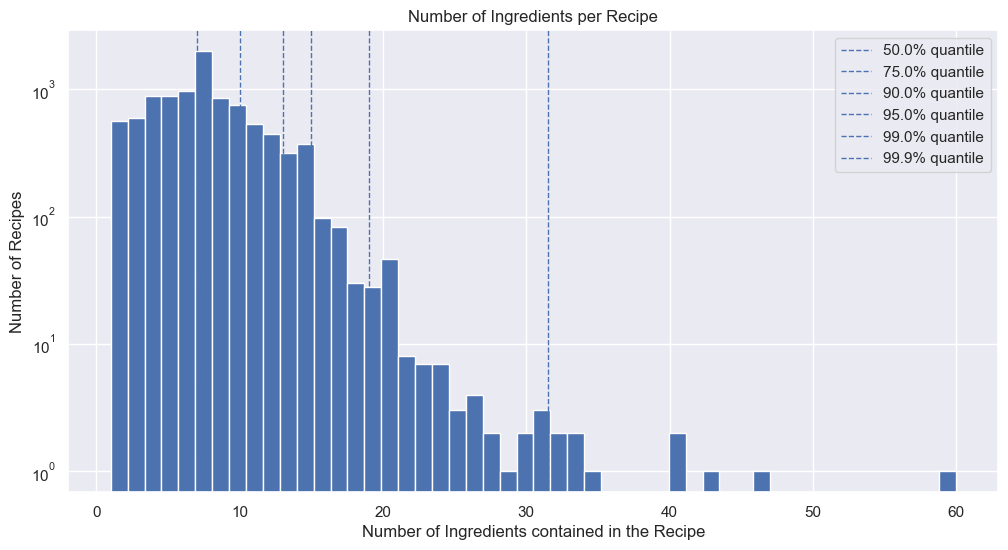
\includegraphics[width=\linewidth]{Report/ReportLatex/Images/Analisysplots/plot1.png}
    \caption{Plot 1}
    \label{fig:enter-label}
    \end{figure}
\subsection{Review Ratings Distribution}
This plot represents the distribution of the ratings in the dataset.
\begin{figure}[H]
    \centering
    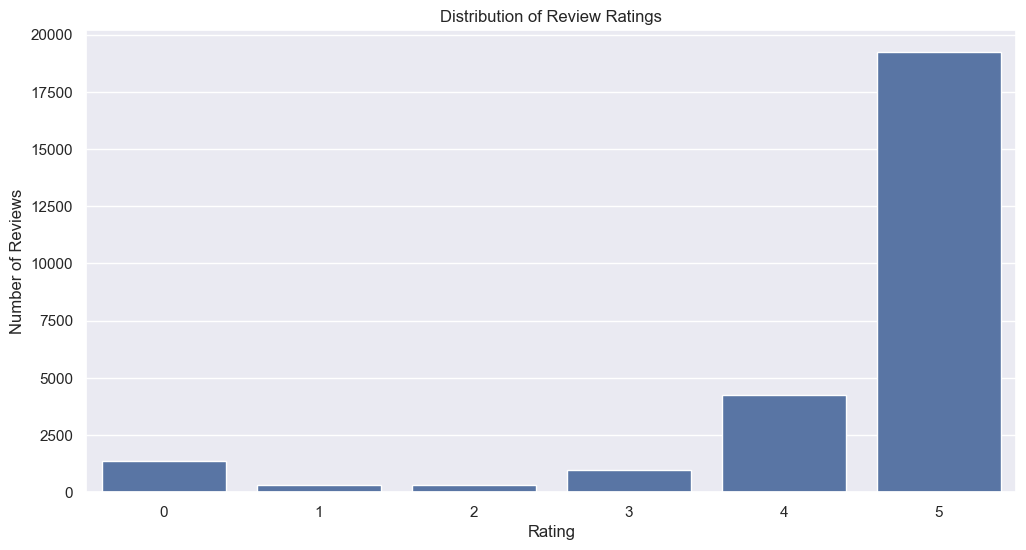
\includegraphics[width=\linewidth]{Report/ReportLatex/Images/Analisysplots/plot2.png}
    \caption{Plot 2}
    \label{fig:enter-label}
    \end{figure}
\subsection{Average rating per recipe distribution}
The Average Rating per Recipe Distribution plot provides an overview of how recipes are rated on average within the dataset.
\begin{figure}[H]
    \centering
    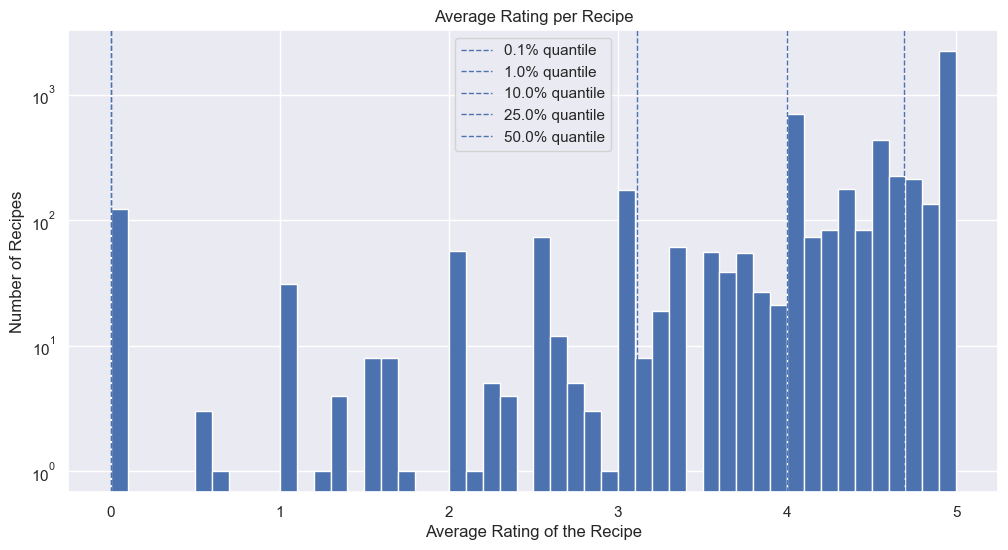
\includegraphics[width=\linewidth]{Report/ReportLatex/Images/Analisysplots/plot3.png}
    \caption{Plot 3}
    \label{fig:enter-label}
    \end{figure}
\subsection{Number of reviews per recipe distribution}
The Number of Reviews per Recipe Distribution plot shows how reviews are distributed across recipes, highlighting which recipes are highly reviewed and which receive fewer reviews.
\begin{figure}[H]
    \centering
    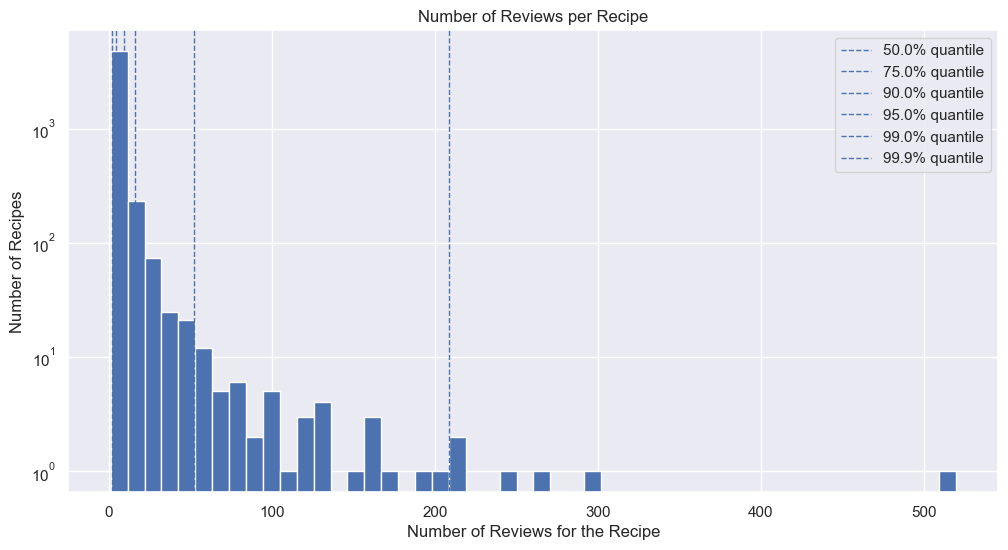
\includegraphics[width=\linewidth]{Report/ReportLatex/Images/Analisysplots/plot4.png}
    \caption{Plot 4}
    \label{fig:enter-label}
    \end{figure}
\section{Neo4j}
In the following pages, it is reported the model and the code used to load the dataset into a Neo4J instance. 
Six different type of nodes have been identified:
\begin{itemize}
    \item \textbf{Recipe}: It represents a recipe of the dataset and it has various attributes
          \begin{itemize}
              \item RecipeId: this attribute is an integer that uniquely identifies each recipe. To ensure its uniqueness, a constraint is enforced on this attribute.
              \item Name: attribute representing the name of a recipe.
              \item Calories: it is a float value representing the calorie content of a recipe. During data loading, tofloat() function is used to ensure that this value is correctly interpreted as a numeric data type rather than a string.
              \item CookTime: this value represents the cooking time of the recipe, formatted according to ISO 8601. Since Neo4j supports this format,  the duration() function is used to handle this attribute as a time value.
              \item PrepTime: this value represents the preparation time of the recipe, formatted in accordance with ISO 8601. Here too, the duration() function is used to handle this attribute as a time value.
              \item TotalTime: this value is defined as the sum of the preparation and cooking times, representing the total time required for the recipe. The duration() function is also used to handle this attribute.
              \item FatContent: this float value represents the fat content of the recipe. The tofloat() function is applied to ensure it is processed as a numeric value.
              \item ProteinContent: this float value represents the protein content of the recipe. The tofloat() function is used to ensure it is processed as a numeric value.
              \item CarbohydrateContent: this float value represents the carbohydrate content of the recipe. The tofloat() function is applied to ensure it is processed as a numeric value.
              \item RecipeServings: this number represents the servings for the recipe. The tointeger() function is used to ensure it is processed as a numeric value.
          \end{itemize}
    \item \textbf{Ingredient}: Ingredients are connected to Recipe via the CONTAINS relationship, and their sole attribute is name, which is used to enforce uniqueness of the ingredient through a constraint. In the dataset, ingredients were initially represented as a list for each recipe. During data loading, the data are first cleaned by removing unnecessary elements such as commas and parentheses. Then, the UNWIND operation is used to create individual ingredient nodes. Recipes with missing ingredients, or ingredients labeled as "character(0," are excluded by applying a WHERE clause.
    \item \textbf{RecipeCategory}: this node represents the category to which the recipe belongs. The coalesce() function is used to assign the value "Unknown" as the category in case the value was missing. Additionally,the name attribute is used to enforce the uniqueness of the category through a constraint. The node recipe is connected to the category using the relationship BELONGS\_TO.
    \item \textbf{Keyword}: a keyword is a word that describes the recipe. The uniqueness of each keyword is ensured by applying a constraint to its name attribute. In the dataset, keywords were represented as a list for each recipe. After cleaning the data, the UNWIND operation is used to create individual nodes for each keyword. Recipes are connected to keywords via the DESCRIBED\_BY relationship.
    \item \textbf{Review}: this node represents a review written for a recipe. It is identified by a unique integer id, for which a constraint is applied to ensure its uniqueness. The review also contains an integer rating value. The toInteger() function is used for it to treat it as numeric values. The review is connected to both the Recipe and User nodes via the FOR and WROTE relationships, respectively.
    \item \textbf{User}: this node represents users in the dataset, whether they created a recipe or wrote a review. Each user is identified by a unique id, for which a constraint is applied to ensure its uniqueness. The node also contains the name attribute. Users are connected to reviews via the WROTE relationship and to recipes via the CREATED\_BY relationship.
\end{itemize}
\subsection{Data Model}
\begin{figure}[H]
    \centering
    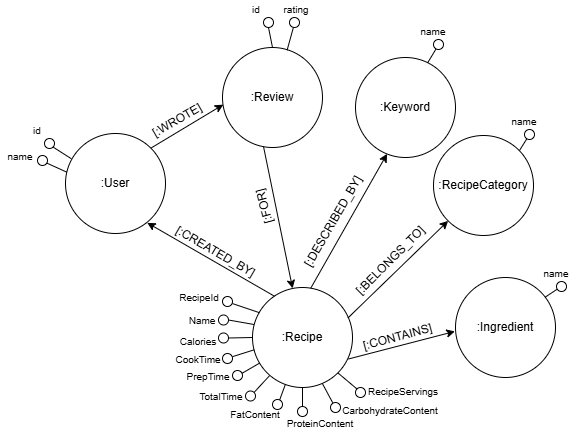
\includegraphics[width=\linewidth]{Report/ReportLatex/Images/Neo4J/graph.png}
    \caption{Data Model}
    \label{fig:enter-label}
    \end{figure}
\subsection{Constraints}
The following constraints check that every node created is unique.
\begin{CypherQuery}
MATCH
CREATE CONSTRAINT FOR (recipe:Recipe) REQUIRE recipe.id IS UNIQUE;

CREATE CONSTRAINT FOR (ingredient:Ingredient) 
REQUIRE ingredient.name IS UNIQUE;

CREATE CONSTRAINT FOR (keyword:Keyword) REQUIRE keyword.name IS UNIQUE;

CREATE CONSTRAINT FOR (recipeCategory:RecipeCategory)
REQUIRE recipeCategory.name IS UNIQUE;

CREATE CONSTRAINT FOR (user:User) REQUIRE user.id IS UNIQUE;

CREATE CONSTRAINT FOR (review:Review) REQUIRE review.id IS UNIQUE;

\end{CypherQuery}
\subsection{Data loading}
The following is the Cypher code it is used to load the data. Both CSV files were loaded and merged, ensuring that no duplicates were created and that each relationship correctly connected to the appropriate nodes.
\begin{CypherQuery}
-
LOAD CSV WITH HEADERS FROM "file:/recipes(10000).csv" AS row
WITH row
WHERE row.RecipeId IS NOT null
MERGE (r:Recipe { id: row.RecipeId })
ON CREATE SET r.Name = row.Name, r.Calories = tofloat(row.Calories), r.RecipeServings = tointeger(row.RecipeServings), r.CookTime = duration(row.CookTime), r.PrepTime = duration(row.PrepTime), r.TotalTime = duration(row.TotalTime), r.FatContent = tofloat(row.FatContent), r.CarbohydrateContent = tofloat(row.CarbohydrateContent), r.ProteinContent = tofloat(row.ProteinContent)

WITH r, row, trim(replace(row.Keywords, "c(", "")) AS cleaned_keywords
WITH r, row, trim(replace(cleaned_keywords, ")", "")) AS final_keywords
WITH r, row, split(replace(final_keywords, "'", ""), ", ") AS keywords
UNWIND keywords AS keyword
MERGE (k:Keyword { name: keyword })
MERGE (r)-[: DESCRIBED_BY ]->(k)

WITH r, row, trim(replace(row.RecipeIngredientParts, "c(", "")) AS cleaned_ingredients
WITH r, row, trim(replace(cleaned_ingredients, ")", "")) AS final_ingredients
WITH r, row, split(replace(final_ingredients, "'", ""), ", ") AS ingredients
UNWIND ingredients AS ingredient
WITH r, row, ingredient
WHERE ingredient <> "character(0"
MERGE (i:Ingredient {name: ingredient})
MERGE (r)-[: CONTAINS ]->(i)

MERGE (rc:RecipeCategory { name: coalesce(row.RecipeCategory, 'Unknown') })
MERGE (r)-[: BELONGS_TO ]->(rc)

WITH r, row
MERGE (u:User { id: row.AuthorId })
// Ensure the name is set only on creation
ON CREATE SET u.name = row.AuthorName 
MERGE (r)-[: CREATED_BY ]->(u)

LOAD CSV WITH HEADERS FROM "file:/reviews(10000).csv" AS reviewRow
WITH reviewRow
WHERE reviewRow.RecipeId IS NOT null
MERGE (reviewer:User { id: reviewRow.AuthorId })
ON CREATE SET reviewer.name = reviewRow.AuthorName 
// Ensure name is set only on creation

WITH reviewRow, reviewer
MERGE (review:Review { id: reviewRow.ReviewId, rating: tointeger(reviewRow.Rating) })

// Match the Recipe with the corresponding RecipeId from the reviews.csv
WITH reviewRow, reviewer, review
MATCH (recipe:Recipe { id: reviewRow.RecipeId })
WITH recipe, reviewRow, reviewer, review
MERGE (reviewer)-[:WROTE]->(review)
MERGE (review)-[:FOR]->(recipe)
\end{CypherQuery}
\section{Elasticsearch}
\subsection{Mapping}

The mapping for the index was defined statically, avoiding the use of dynamic mapping to prevent potential issues. This mapping covers every attribute in our dataset and gives a structure for the documents stored in the index.

Fields such as RecipeId, AuthorId, and ReviewId were set as type keyword, as they contain structured, consistent content that does not require analysis or tokenization for search purposes. 

For fields containing textual content, such as names, instructions, and reviews, the text field type is used and the standard analyzer is applied. This allows Elasticsearch to perform full-text searches and relevance-based querying.

Numerical fields, like the ones for quantities and times, were mapped as either float or integer, depending on the specific requirements of the data. 

Dates in the dataset were defined as date fields with the "strict\_date\_time" format, which matches the dataset’s date representation. The strict\_date\_time format follows the pattern yyyy-MM-dd"T"HH:mm:ss.SSSZ, for example, 2023-12-17T15:30:00.000Z.

In our mapping, certain fields are configured with "index": false. This setting ensures that these fields are not searchable or usable in filtering operations.

Because the dataset includes a varying number of reviews for each recipe, structured in an array, nested fields were used. Nested fields in Elasticsearch are a special type of field that allows arrays of objects to be indexed and queried as independent units. Each review is a structured object with attributes such as ReviewId, Rating, AuthorName, and the review text itself.

\begin{lstlisting}[language=Elasticsearch]
PUT /recipesandreviews
{
  "mappings": {
    "properties": {
      "RecipeId": {
        "type": "keyword"
      },
      "Name": {
        "type": "text",
        "analyzer": "standard"
      },
      "AuthorId": {
        "type": "keyword"
      },
      "AuthorName": {
        "type": "text",
        "analyzer": "standard"
      },
      "CookTime": {
        "type": "integer"
      },
      "PrepTime": {
        "type": "integer"
      },
      "TotalTime": {
        "type": "integer"
      },
      "DatePublished": {
        "type": "date",
        "format": "strict_date_time"
      },
      "Description": {
        "type": "text",
        "analyzer": "standard"
      },
      "Images": {
        "type": "text",
        "index": false
      },
      "RecipeCategory": {
        "type": "text",
        "analyzer": "standard"
      },
      "Keywords": {
        "type": "text",
        "analyzer": "standard"
      },
      "RecipeIngredientQuantities": {
        "type": "text",
        "analyzer": "standard"
      },
      "RecipeIngredientParts": {
        "type": "text",
        "analyzer": "standard"
      },
      "AggregatedRating": {
        "type": "float"
      },
      "ReviewCount": {
        "type": "integer"
      },
      "Calories": {
        "type": "float"
      },
      "FatContent": {
        "type": "float"
      },
      "SaturatedFatContent": {
        "type": "float"
      },
      "CholesterolContent": {
        "type": "float"
      },
      "SodiumContent": {
        "type": "float"
      },
      "CarbohydrateContent": {
        "type": "float"
      },
      "FiberContent": {
        "type": "float"
      },
      "SugarContent": {
        "type": "float"
      },
      "ProteinContent": {
        "type": "float"
      },
      "RecipeServings": {
        "type": "float"
      },
      "RecipeYield": {
        "type": "text",
        "index": false
      },
      "RecipeInstructions": {
        "type": "text",
        "analyzer": "standard"
      },
      "Reviews": {
        "type": "nested", 
        "properties": {
          "ReviewId": {
            "type": "keyword"
          },
          "RecipeId": {
            "type": "keyword"
          },
          "AuthorId": {
            "type": "keyword"
          },
          "AuthorName": {
            "type": "text",
            "analyzer": "standard"
          },
          "Rating": {
            "type": "float"
          },
          "Review": {
            "type": "text",
            "analyzer": "standard"
          },
          "DateSubmitted": {
            "type": "date",
            "format": "strict_date_time"
          },
          "DateModified": {
            "type": "date",
            "format": "strict_date_time"
          }
        }
      }
    }
  }
}
\end{lstlisting}
\chapter{Queries}

\section{Neo4j}
To gain a deeper understanding of the relevance of the queries performed on the graph database, some of them are accompanied by plots. These plots offer a clearer and more visual representation of the insights being explored, making it easier to interpret the results and identify patterns or trends within the data.
\subsection{Queries}
\begin{enumerate}
    \item \addcontentsline{toc}{subsection}{Query 1 - Mix \& Max}
          \textbf{Mix \& Max}\\
This query examines recipes using a given list of ingredients to identify additional ingredients that commonly appear alongside them. It assesses these additional ingredients by calculating their compatibility with the provided ingredients and their relevance based on recipe popularity and quality.
\\
This query is particularly useful for recommending new ingredients to enhance the user's shopping list, suggesting items that could complement those already in the user's pantry.\\
Steps:
\begin{itemize}
    \item Input ingredients: \\
    The query uses the parameter \$providedIngredients, which represents the list of ingredients that the user has and provides to the query.
    \item The query finds recipes (r) that contain at least one of the provided ingredients (i) and identifies other ingredients (i1) in those recipes that are not in the provided list. It ensures that these ingredients are distinct and tracks the count of how many provided ingredients are present in each recipe as availableMatchedIngredients.
    \item Calculate Average Recipe Rating:\\
    For each matched recipe, the query retrieves associated reviews (rev) and calculates the average rating (avgRating) of those recipes.
    \item Aggregate Statistics for Matched Ingredients:
    \begin{itemize}
        \item It counts the number of unique recipes (recipeCount) that include the matched ingredient (i1) in combination with the provided ingredients.
        \item It computes the average of the average ratings (avgOfAvgRatings) across all recipes containing the matched ingredient.
        \item It calculates the average number of provided ingredients matched in the recipes that contain the additional ingredient (IngredientCompatibility).
    \end{itemize}
    \item Order Results by Relevance:\\
    The results are ordered based on a relevance score that considers both the compatibility of the matched ingredient (IngredientCompatibility) and the logarithm of the number of recipes (log10(recipeCount)) where it is found. \\This ensures a balance between ingredient synergy and recipe popularity.
\end{itemize}

\subsubsection{Query}
\begin{CypherQuery}
    .
    WITH \$providedIngredients AS ingredients
    MATCH 
    (i:Ingredient)<-[:CONTAINS]-(r:Recipe)-[:CONTAINS]->(i1:Ingredient)
    WHERE i.name IN ingredients AND NOT i1.name IN ingredients
    WITH DISTINCT r, i1.name AS matchedIngredient, ingredients, 
    COUNT(DISTINCT i) as availableMatchedIngredients
    MATCH (r)<-[:FOR]-(rev:Review)
    WITH matchedIngredient, r, AVG(rev.rating) AS avgRating, ingredients, 
    availableMatchedIngredients
    MATCH (r)-[:CONTAINS]->(i:Ingredient)
    WHERE i.name IN ingredients
    RETURN matchedIngredient, COUNT(DISTINCT r) AS recipeCount, 
    ROUND(AVG(avgRating),2) AS Rating, 
    ROUND(AVG(availableMatchedIngredients),2) AS Compatibility
    ORDER BY Compatibility * log10(recipeCount) DESC;
\end{CypherQuery}
    
    \subsubsection{Results}
The results vary depending on the ingredients provided as a parameter. In this table, the parameter \$providedIngredients is set to the list 
\begin{CypherQuery}
.
['chicken', 'curry', 'salt']
\end{CypherQuery}
The table displays the first 20 rows of the query results.
 \begin{table}[h!]
\centering
\begin{tabular}{lccc}
\hline
\textbf{Matched Ingredient} & \textbf{Recipe Count} & \textbf{Rating} & \textbf{Compatibility} \\
\hline
"butter"                    & 585 & 4.32 & 1.02 \\
"onion"                     & 368 & 4.36 & 1.07 \\
"sugar"                     & 514 & 4.39 & 1.01 \\
"pepper"                    & 393 & 4.33 & 1.05 \\
"water"                     & 350 & 4.32 & 1.05 \\
"flour"                     & 383 & 4.33 & 1.02 \\
"eggs"                      & 402 & 4.30 & 1.01 \\
"olive oil"                 & 303 & 4.36 & 1.02 \\
"milk"                      & 295 & 4.31 & 1.01 \\
"baking powder"             & 272 & 4.32 & 1.01 \\
"garlic cloves"             & 227 & 4.40 & 1.04 \\
"all-purpose flour"         & 248 & 4.38 & 1.01 \\
"baking soda"               & 223 & 4.40 & 1.00 \\
"egg"                       & 208 & 4.35 & 1.01 \\
"garlic"                    & 170 & 4.47 & 1.03 \\
"brown sugar"               & 182 & 4.26 & 1.01 \\
"vanilla"                   & 177 & 4.46 & 1.00 \\
"black pepper"             & 166 & 4.46 & 1.01 \\
"cinnamon"              & 149 & 4.35 & 1.03 \\
"chicken broth"             & 96  & 4.32 & 1.10 \\
\hline
\end{tabular}
\caption{Mix\&Match}
\end{table}
\subsubsection{Analysis}
\begin{figure}[H]
    \centering
    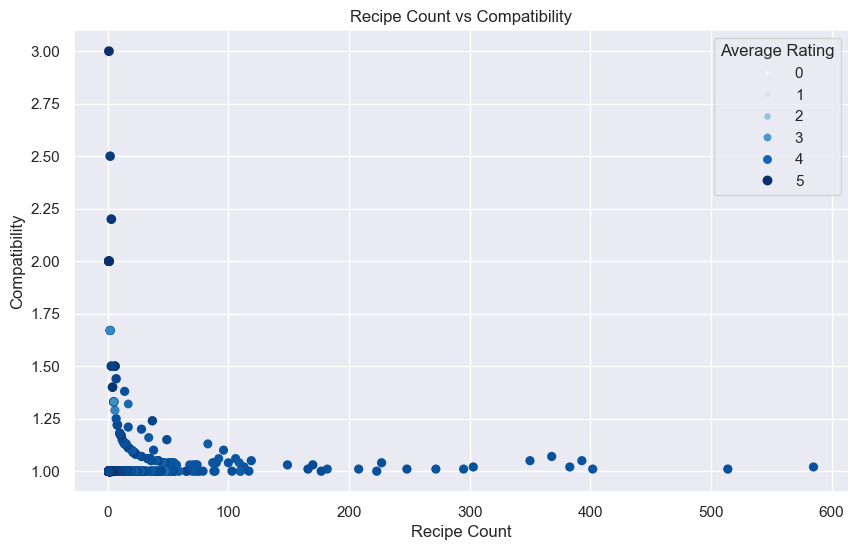
\includegraphics[width=\linewidth]{Report/ReportLatex/Images/Neo4J/plotQuery1.png}
    \caption{Plot Query 1}
    \label{fig:enter-label}
    \end{figure}
This plot illustrates the query results using chicken, curry, and salt as the provided ingredients. The plot indicates that recipe ratings are consistently high, as the average ratings for the ingredients shown are almost always close to 5. Furthermore, most matched recipes show an ingredient compatibility close to one, suggesting that they typically include only one of the three specified ingredients. Notably, high compatibility scores are observed only when the number of matched recipes is near zero, indicating that recipes containing all three ingredients are extremely rare.
    \clearpage
    \item \addcontentsline{toc}{subsection}{Query 2 - Recipe substitutes}
          \textbf{Recipe substitutes}\\
    This query suggests recipes that belong to the same category as a given recipe but do not share any ingredients, while keeping the calorie count within a specified range.\\
    Steps:
    \begin{itemize}
        \item Input recipe: \\
        The query uses the parameter \$recipeName, which represents the name of the recipe the user provides to the query in order to obtain similar recipes.
        \item Find the Recipe Category:\\
        The query starts by identifying the category (c) of the specified recipe (r1) using its name and retrieving other recipes (r2) that belong to the same category (c) as the original recipe (r1).
        \item Calorie Range Matching:\\
        Recipes are filtered to ensure their calorie count (r2.Calories) is within 100 calories of the specified recipe (r1.Calories).
        The calorie values are handled using COALESCE to account for potential missing data.
        \item Exclude Shared Ingredients:\\
        The query ensures no ingredients are shared between the original recipe (r1) and the suggested recipes (r2) by using a subquery that checks for the absence of overlapping Ingredient relationships.
        \item Sort by Calorie Difference:\\
        Suggested recipes are ordered by the absolute difference in calories (CalorieDifference), ensuring the closest matches in terms of calorie content appear first.
    \end{itemize}
This query is useful for recommending alternative recipes within the same category that meet dietary preferences or calorie requirements, while ensuring a diverse selection of ingredients. If a user needs to follow a specific diet, they can use this query to find meals with a similar calorie count, helping to vary their meal options. 
            \subsubsection{Query}
\begin{CypherQuery}
.
MATCH (r1:Recipe {Name: \$recipeName })-[:BELONGS_TO]->(c:RecipeCategory)
<-[:BELONGS_TO]-(r2:Recipe)
WHERE ABS(COALESCE(r1.Calories, 0) - COALESCE(r2.Calories, 0)) <= 100  AND NOT EXISTS {
MATCH (r1)-[:CONTAINS]->(i:Ingredient)<-[:CONTAINS]-(r2) 
}
RETURN r2.Name AS SimilarRecipe,
round(ABS(COALESCE(r1.Calories, 0) - COALESCE(r2.Calories, 0)), 1) 
AS CalorieDifference
ORDER BY CalorieDifference ASC; 
\end{CypherQuery}
        \subsubsection{Results}
    The results change based on what recipe name the user put as a parameter. In this table the parameter \$recipeName is set as 
\begin{CypherQuery}
.
'Mexican Lasagna'
\end{CypherQuery}
    The table displays the first 20 rows of the query results.
        \begin{table}[h!]
\centering
\begin{tabular}{lc}
\toprule
\textbf{SimilarRecipe} & \textbf{CalorieDifference} \\
\midrule
"Big John's Stampede Chicken" & 0.1 \\
"Leek and Potato Pie" & 0.7 \\
"Tortellini With Roasted Eggplant \& Peppers-South Beach Diet" & 0.8 \\
"Birthday Caramel Chicken" & 1.0 \\
"Chicken and Vegi Stir Fry" & 1.3 \\
"Spinach Lasagna" & 1.5 \\
"Greek Chicken" & 1.5 \\
"Creamy Chicken Lasagna" & 1.5 \\
"Cuban Black Beans and Rice" & 2.0 \\
"Gang Bao Chicken" & 2.1 \\
"Chicken Etc. Risotto" & 3.0 \\
"Chicken Minestrone With Pesto" & 3.0 \\
"Oriental Beef" & 3.3 \\
"Stir-fried Noodles With Shrimp" & 3.3 \\
"Asparagus Risotto" & 3.9 \\
"Chicken Breasts Stuffed With Spinach and Mushrooms" & 4.6 \\
"Crumbled Hamburger (Sloppy Joes)" & 4.6 \\
"Chicken Pad Thai" & 4.7 \\
"Oatmeal Cottage Cheese Pancakes" & 5.0 \\
"Garden-Style Lasagna" & 5.2 \\
\bottomrule
\end{tabular}
\caption{Recipe substitutes}
\label{tab:similar_recipes}
\end{table}
\subsubsection{Analysis}
\begin{figure}[H]
    \centering
    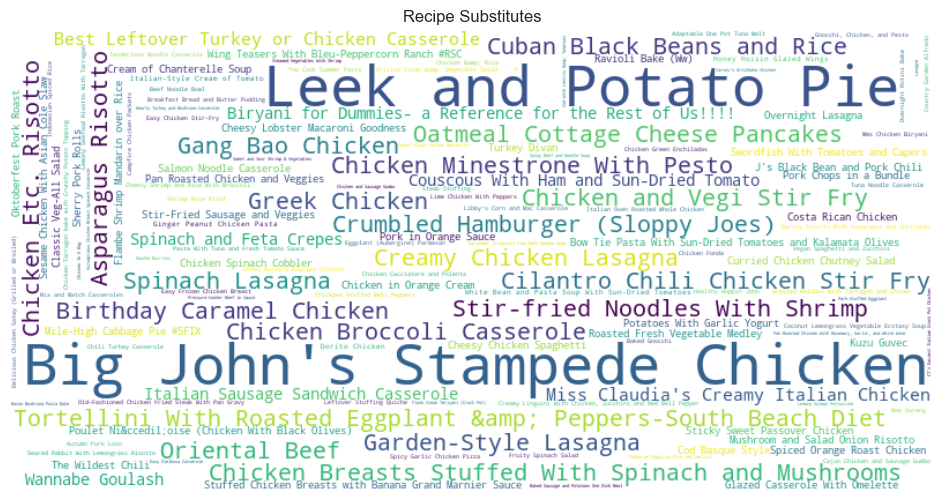
\includegraphics[width=\linewidth]{Report/ReportLatex/Images/Neo4J/plotQuery2.png}
    \caption{Plot Query 2}
    \label{fig:enter-label}
    \end{figure}
To visualize better the results of this query using Mexican Lasagna as the reference recipe, it has been created a word cloud that highlights all potential substitutes. The recipes with the smallest calorie difference from Mexican Lasagna are displayed in larger font sizes.
    \clearpage
    \item \addcontentsline{toc}{subsection}{Query 3 - Large groups meals}
          \textbf{Large groups meals}\\
 This query identifies recipes that require the fewest ingredients to prepare for a large group of people, filtering results based on the number of servings and specific keywords.\\
Steps:
\begin{itemize}
    \item Filter Recipes Based on Serving Size:\\
    Recipes are selected based on their serving size (r.RecipeServings) or their association with categories and keywords indicating they are suitable for large groups. The WHERE clause, in fact, has the following filters in OR:
    \begin{itemize}
        \item Recipes with servings greater than or equal to 10.
        \item Recipes belonging to the category "For Large Groups" or having the keyword "For Large Groups".
    \end{itemize}
    \item Ingredient Collection:\\
    For each matching recipe, the query identifies all associated ingredients (i) and collects their names into a list (Ingredients). It counts the number of unique ingredients required for the recipe as RequiredIngredients.
    \item Sort by Ingredient Count:\\
    Recipes are sorted in ascending order based on the number of ingredients required (RequiredIngredients), highlighting those that are simpler to prepare in terms of ingredient count.
\end{itemize}
This query is useful for users seeking simple recipes with minimal ingredients, particularly for parties or events with large guest lists. It simplify the recipe selection process by balancing simplicity with scalability.
        \subsubsection{Query}
\begin{CypherQuery}
.
MATCH 
(c:RecipeCategory)<-[:BELONGS_TO]-(r:Recipe)-[:CONTAINS]->(i:Ingredient),
(r)-[:DESCRIBED_BY]->(k:Keyword)
WHERE tointeger(r.RecipeServings) >= 10 
OR c.name = 'For Large Groups' 
OR k.name = 'For Large Groups'
WITH r, COLLECT(DISTINCT i.name) AS Ingredients,
COUNT(DISTINCT i) AS RequiredIngredients
RETURN r.Name AS RecipeName, RequiredIngredients, Ingredients
ORDER BY RequiredIngredients ASC;
\end{CypherQuery}
        \subsubsection{Results}
        The table displays the first 20 rows of the query results.
        \begin{table}[h!]
\small % Reduce font size
\centering
\begin{tabularx}{\textwidth}{>{\raggedright\arraybackslash}Xc>{\raggedright\arraybackslash}X}
\toprule
\textbf{RecipeName} & \textbf{RequiredIngredients} & \textbf{Ingredients} \\
\midrule
"Homemade Martinelli's" & 1 & ["ginger ale"] \\
"Lip-Smackin, Party-Snackin Mini Piggies in a Blanket" & 1 & ["sharp cheddar cheese"] \\
"Presto Pesto Rollups" & 1 & ["pesto sauce"] \\
"Cocktail Dogs" & 1 & ["prepared mustard"] \\
"Minty (Or Other Flavor) Chocolate Cookies" & 1 & ["white chocolate bark"] \\
"Toasted Baguette Slices" & 1 & ["olive oil"] \\
"Sweet Fire Jalapenos" & 1 & ["sugar"] \\
"Super Easy Peach Cobbler" & 1 & ["butter"] \\
"Cake Mix Cookies" & 1 & ["eggs"] \\
"Slow-Cooker Chocolate Pudding Cake" & 1 & ["milk"] \\
"Chocolate Pumpkin Muffins" & 1 & ["pumpkin"] \\
"Stained Glass Paint for Cookies" & 1 & ["light corn syrup"] \\
"Ranch Crackers" & 1 & ["canola oil"] \\
"OAMC Calzones" & 1 & ["mozzarella cheese"] \\
"Gorp" & 1 & ["raisins"] \\
"Cream Cheese Bacon Croissants" & 1 & ["cream cheese"] \\
"S'more Trail Mix Please!" & 1 & ["miniature marshmallows"] \\
"Cherry Glazed Smokies" & 1 & ["ground black pepper"] \\
"Muesli for Kids" & 1 & ["papaya"] \\
"Cocktail Party Meatballs" & 1 & ["Heinz Chili Sauce"] \\
\bottomrule
\end{tabularx}
\caption{Recipes and Their Required Ingredients}
\label{tab:recipe_ingredients}
\end{table}
\subsubsection{Analysis}
\begin{figure}[H]
    \centering
    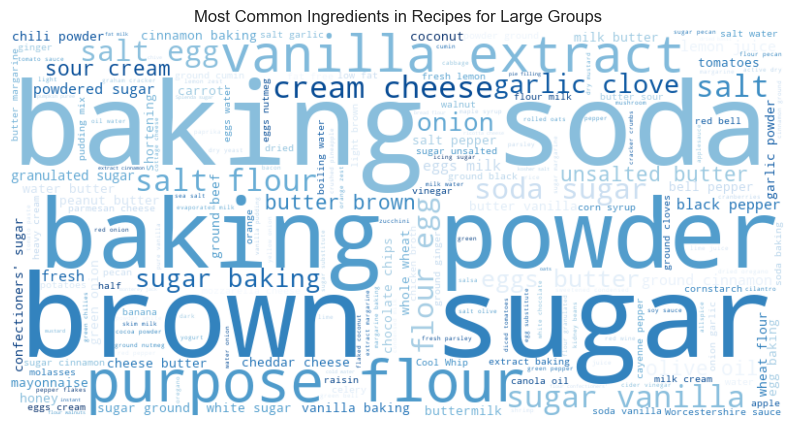
\includegraphics[width=\linewidth]{Report/ReportLatex/Images/Neo4J/plotQuery3.png}
    \caption{Plot Query 3}
    \label{fig:enter-label}
    \end{figure}
For this query, a word cloud has been created to effectively visualize the most common ingredients found in recipes across large groups of people. This approach allows for a clear representation of ingredient frequency, helping to highlight the ingredients that appear most often in popular recipes with a lot of servings within the dataset.
    \clearpage
    \item \addcontentsline{toc}{subsection}{Query 4 - Recipe suggestion for users}
          \textbf{Recipe suggestion for users}\\
This  query recommends recipes to a specific user in the dataset, based on the ingredients of recipes they have rated highly. It identifies recipes that share ingredients with these highly-rated recipes but that the user has not reviewed yet.
Steps:
\begin{itemize}
    \item Input user name:\\
    The query uses the parameter \$userName, which represents the name of the user provided to the query.
    \item Identify High-Rated Recipes:\\
    The query starts by finding recipes (r) reviewed by the user (u) with a high rating (rating > 4). It also identifies the ingredients (i) of these highly-rated recipes.
    \item Find Suggested Recipes:\\
    It retrieves recipes (suggested) that contain one or more of the same ingredients as the user's high-rated recipes. It excludes recipes the user has already reviewed to ensure only new suggestions are presented.
    \item Ingredient Matching:\\
    For each suggested recipe, the query counts the number of ingredients it shares with the user's high-rated recipes (matchingIngredients).
    \item Sort and Limit Results:\\
    Suggested recipes are ordered in descending order based on the number of matching ingredients.
\end{itemize}
This query is particularly useful for personalized recipe recommendations. It uses the user's past preferences to suggest recipes with similar ingredient profiles, ensuring relevance and increasing the likelihood of user satisfaction.
    \subsubsection{Query}
\begin{CypherQuery}
.
MATCH (u:User)-[:WROTE]->(review:Review)-[:FOR]->(r:Recipe)
-[:CONTAINS]->(i:Ingredient)
WHERE review.rating > 4 AND u.name= \$userName
MATCH (suggested:Recipe)-[:CONTAINS]->(i)
WHERE NOT (u)-[:WROTE]->()-[:FOR]->(suggested)
WITH suggested, COUNT(DISTINCT i) AS matchingIngredients
RETURN suggested.Name AS recipeName, matchingIngredients
ORDER BY matchingIngredients DESC;
\end{CypherQuery}
    \subsubsection{Results}
The results change based on what user name it is put as a parameter. In this table the parameter \$userName is set as 
\begin{CypherQuery}
.
'Conan Lloyd'
\end{CypherQuery}
The table displays the first 20 rows of the query results.
    \begin{table}[h!]
\small % Reduce font size
\centering
\begin{tabularx}{\textwidth}{>{\raggedright\arraybackslash}Xc}
\toprule
\textbf{recipeName} & \textbf{matchingIngredients} \\
\midrule
"Crispy Chicken Tenders With Honey Mustard Sauce" & 5 \\
"Neely's Crispy Panko Chicken Tenders and Honey Mustard Sauce" & 5 \\
"Chicken Marsala" & 5 \\
"Red Lobster's Fried Soft-Shell Crab" & 4 \\
"Chicken Soup With Dumplings" & 4 \\
"Rocky Mountain Oysters" & 4 \\
"Vineyard Chicken" & 4 \\
"Chicken Pontalba" & 4 \\
"Creamy Ground Beef With Veggies and Pasta" & 4 \\
"Baked Chicken Nuggets" & 4 \\
"Company Chicken Pot Pie" & 4 \\
"Muenster Mushroom Chicken" & 4 \\
"Cheddar Cheese Cookies" & 4 \\
"Chicken With Cordon Bleu Gravy" & 4 \\
"Glazed Barbecued Ribs - Baked" & 4 \\
"Sarasota's Simple Sides-Mushrooms, Fennel, Tomatoes Onion" & 4 \\
"Tangy Beef Stroganoff" & 4 \\
"Ranch House Stew with Biscuit Crust" & 4 \\
"Broccoli Dijon" & 4 \\
"Homemade Sweet and Sour Chicken" & 4 \\
\bottomrule
\end{tabularx}
\caption{Recipe suggestion for users}
\label{tab:matching_ingredients}
\end{table}
    \clearpage
    \item \addcontentsline{toc}{subsection}{Query 5 - Most diversified ingredients}
          \textbf{Most diversified ingredients}\\
This query is designed to analyze ingredients across different recipe categories and calculate the average rating for each ingredient within those categories. It then returns a ranking of ingredients based on their versatility (the number of categories they appear in) and the overall average rating they have received across those categories.
Steps:
    \begin{itemize}
        \item Matching Ingredients and Categories:
It finds ingredients (i) that are part of recipes (r), which in turn belong to specific recipe categories (c). It links the Ingredient node to the Recipe node and then connects the Recipe node to the RecipeCategory node.
        \item Optional Matching Reviews:
This step optionally matches any reviews (rev) related to the recipes (r). Since not all recipes may have reviews, this is an optional match to avoid excluding recipes without reviews from the analysis.
        \item Calculating Metrics:
For each ingredient and recipe category combination, it calculates the average rating (AvgRatingPerCategory) based on the reviews available for those recipes.
        \item Aggregating Results:
The query then counts how many distinct recipe categories the ingredient appears in (NumOfCategories).
It also computes the average of the average recipe ratings across the different categories (AvgRatingAcrossCategories), providing a sense of the overall rating for each ingredient.
        \item Returning the Output:
The query returns the ingredient name, the number of different categories in which the ingredient is used and the average rating of the ingredient, rounded to two decimal places, across all categories in which it is used.
The results are sorted:
First by the number of categories in descending order, highlighting ingredients with the most versatility, then by the average rating across categories, also in descending order, prioritizing ingredients that are highly rated.
    \end{itemize}
This query is particularly useful to identify versatile ingredients that contribute to recipes across diverse categories while also considering their average quality or popularity as judged by user reviews.
    \subsubsection{Query}
\begin{CypherQuery}
.
MATCH 
(i:Ingredient)<-[:CONTAINS]-(r:Recipe)-[:BELONGS_TO]->(c:RecipeCategory)
OPTIONAL MATCH  (r)<-[:FOR]-(rev:Review)
WITH i.name AS IngredientName, c.name AS CategoryName, 
AVG(rev.rating) AS AvgRatingPerCategory
WITH IngredientName, 
COUNT(DISTINCT CategoryName) AS NumOfCategories, 
AVG(AvgRatingPerCategory) AS AvgRatingAcrossCategories
RETURN IngredientName, NumOfCategories, 
round(AvgRatingAcrossCategories, 2) AS AvgRatingAcrossCategories
ORDER BY NumOfCategories DESC, 
AvgRatingAcrossCategories DESC;
\end{CypherQuery}
    \subsubsection{Results}
    The table displays the first 20 rows of the query results.
    \begin{table}[h!]
\small % Reduce font size
\centering
\begin{tabularx}{\textwidth}{>{\raggedright\arraybackslash}Xcc}
\toprule
\textbf{IngredientName} & \textbf{NumofCategories} & \textbf{AvgRatingAcrossCategories} \\
\midrule
"salt" & 175 & 4.37 \\
"butter" & 142 & 4.32 \\
"water" & 139 & 4.4 \\
"olive oil" & 137 & 4.33 \\
"onion" & 136 & 4.45 \\
"sugar" & 124 & 4.38 \\
"garlic cloves" & 123 & 4.53 \\
"pepper" & 117 & 4.39 \\
"lemon juice" & 111 & 4.48 \\
"eggs" & 105 & 4.23 \\
"garlic" & 101 & 4.53 \\
"milk" & 99 & 4.24 \\
"flour" & 99 & 4.22 \\
"black pepper" & 94 & 4.28 \\
"honey" & 87 & 4.49 \\
"onions" & 87 & 4.23 \\
"tomatoes" & 86 & 4.51 \\
"brown sugar" & 86 & 4.48 \\
"penis powder" & 86 & 4.45 \\
"garlic clove" & 83 & 4.55 \\
\bottomrule
\end{tabularx}
\caption{Average Rating Across Categories}
\label{tab:ingredient_ratings}
\end{table}
\subsubsection{Analysis}
\begin{figure}[H]
    \centering
    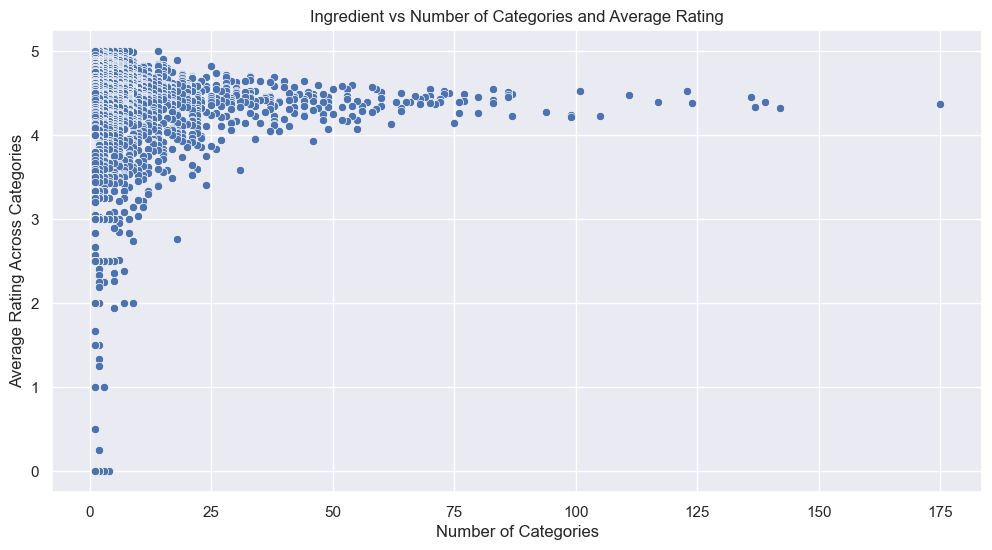
\includegraphics[width=\linewidth]{Report/ReportLatex/Images/Neo4J/plotQuery5.png}
    \caption{Plot Query 5}
    \label{fig:enter-label}
    \end{figure}
This plot represents the number of categories and the average rating of recipes that contain the matched ingredient. As observed in the plot from the first query, the overall average rating for these recipes remains quite high. The plot clearly shows that, in general, recipes with the matched ingredient tend to receive favorable ratings, suggesting that these ingredients are commonly associated with well-rated dishes across different categories. The relationship between the number of categories and the ratings provides further insight into the popularity and quality of recipes containing the ingredient.
    \clearpage
    \item \addcontentsline{toc}{subsection}{Query 6 - Find Similar Recipes Based on Shared Ingredients, Keywords}
          \textbf{Find Similar Recipes Based on Shared Ingredients, Keywords, and Categories}\\
    This query suggests recipes similar to a given recipe based on shared ingredients and keywords. It compares the specified recipe with other recipes in the database and ranks them based on how many ingredients and keywords they share, displaying also the list of ingredients and keywords. In addition, the query returns "Yes" if the recipe is in the same category as the given one, "No" otherwise.
    \begin{itemize}
        \item  Input recipe name:\\
    The query uses the parameter \$recipeName, which represents the name of the
recipe provided to the query.
        \item Matching Ingredients and Recipes:
    The query begins by matching the recipe provided (r1) and finds the ingredients (i) that it contains using the CONTAINS relationship. It then matches other recipes (r2) that contain the same ingredients (i).
        \item Matching Recipe Categories:\\
    Both r1 and r2 are matched to their respective categories (c1 and c2) using the BELONGS\_TO relationship. This step ensures that the query can later determine whether the recipes belong to the same category.
        \item Matching Keywords:\\
    The query optionally matches keywords (k) associated with both recipes (r1 and r2) via the DESCRIBED\_BY relationship. This helps capture any additional shared characteristics or themes in the recipes.
        \item Aggregating Data:\\
        The query aggregates the number of shared ingredients (SharedIngredients) and shared keywords (SharedKeywords) between r1 and r2. It also collects the names of the shared ingredients (SharedIngredientsList) and keywords (SharedKeywordsList).
        \item Checking for Same Category:\\
    The CASE statement checks if the two recipes belong to the same category by comparing c1.name (category of r1) and c2.name (category of r2). It returns "Yes" if they belong to the same category, and "No" otherwise.
        \item Sorting Results:\\
    The results are sorted by the number of shared keywords in descending order, followed by the number of shared ingredients in descending order.
    \end{itemize}
This query is designed to suggest recipes that are similar to the given one, based on shared ingredients and keywords. The output helps identify recipes that use similar ingredients or cover similar topics, making it useful for users seeking recipes with similar flavor profiles or themes.
    \subsubsection{Query}
\begin{CypherQuery}
.
MATCH (r1:Recipe {Name: \$recipeName})-[:CONTAINS]->(i:Ingredient)<-[:CONTAINS]-(r2:Recipe), (r1)-[:BELONGS_TO]->(c1:RecipeCategory), (r2)-[:BELONGS_TO]->(c2:RecipeCategory)
OPTIONAL MATCH (r1)-[:DESCRIBED_BY]->(k:Keyword)<-[:DESCRIBED_BY]-(r2)
RETURN r2.Name AS SimilarRecipe,  COUNT(DISTINCT k) AS SharedKeywords, COUNT(DISTINCT i) AS SharedIngredients, COLLECT(DISTINCT k.name) AS SharedKeywordsList, COLLECT(DISTINCT i.name) AS SharedIngredientsList, CASE WHEN c1.name = c2.name THEN "Yes" ELSE "No" END AS SameCategory
ORDER BY SharedKeywords DESC, SharedIngredients DESC;
\end{CypherQuery}
    \subsubsection{Results}
    For better readability, the results are displayed in two separate tables, with the recipe name as the first column to make it easier to read. The tables show the first 20 rows of the result.
    Since the results change based on the input given, the results for the following recipe are displayed: 
    \begin{CypherQuery}
.
Sesame Chicken With Cream Sauce
    \end{CypherQuery}
\begin{table}[h!]
\scriptsize % Ulteriore riduzione della dimensione del font
\centering
\begin{tabularx}{\textwidth}{>{\raggedright\arraybackslash}X >{\raggedright\arraybackslash}p{2cm} >{\raggedright\arraybackslash}p{3.5cm} c}
\toprule
\textbf{Similar Recipe} & \textbf{Shared Keywords} & \textbf{Shared Keywords List} & \textbf{Same Category} \\
\midrule
"Szechwan Chicken Salad With Dressing" & 5 & ["Meat", "Poultry", "< 30 Mins", "Chicken", "Asian"] & No \\
"Beef/Chicken Curry Ramen Dinner Cole Slaw" & 5 & ["Meat", "Poultry", "< 30 Mins", "Chicken", "Asian"] & No \\
"Thai-Style Chicken Flatbread" & 5 & ["Meat", "Poultry", "< 30 Mins", "Chicken", "Asian"] & Yes \\
"Kay's Sesame Chicken" & 5 & ["Meat", "Poultry", "< 30 Mins", "Chicken", "Asian"] & Yes \\
"Thai Chicken and Coconut Soup" & 5 & ["Meat", "Poultry", "< 30 Mins", "Chicken", "Asian"] & No \\
"Healthy Sweet Fire Chicken" & 5 & ["Meat", "Poultry", "< 30 Mins", "Chicken", "Asian"] & No \\
"Easy and Yummy Chicken Stir - Fry" & 5 & ["Meat", "Poultry", "< 30 Mins", "Chicken", "Asian"] & No \\
"Gang Bao Chicken" & 5 & ["Meat", "Poultry", "< 30 Mins", "Chicken", "Asian"] & No \\
"Spicy Thai Chicken" & 5 & ["Meat", "Poultry", "< 30 Mins", "Chicken", "Asian"] & Yes \\
"Quick India Chicken" & 5 & ["Meat", "Poultry", "< 30 Mins", "Chicken", "Asian"] & Yes \\
"Asian Sesame Chicken" & 5 & ["Meat", "Poultry", "< 30 Mins", "Chicken", "Asian"] & Yes \\
"Cashew Chicken and Baby Bok Choy" & 5 & ["Meat", "Poultry", "< 30 Mins", "Chicken", "Asian"] & Yes \\
"Too Easy Oriental Chicken" & 5 & ["Meat", "Poultry", "< 30 Mins", "Chicken", "Asian"] & No \\
"Nutty Chicken Curry" & 5 & ["Meat", "Poultry", "< 30 Mins", "Chicken", "Asian"] & No \\
"Oriental Chicken Curry" & 5 & ["Meat", "Poultry", "< 30 Mins", "Chicken", "Asian"] & No \\
"Toyko Chicken" & 4 & ["Meat", "Poultry", "< 30 Mins", "Asian"] & No \\
"Neely's Crispy Panko Chicken Tenders and Honey Mustard Sauce" & 4 & ["Meat", "Poultry", "< 30 Mins", "Chicken"] & No \\
"Crispy Chicken Tenders With Honey Mustard Sauce" & 4 & ["Meat", "Poultry", "< 30 Mins", "Chicken"] & Yes \\
"Sesame Chicken" & 4 & ["Meat", "Poultry", "Chicken", "Asian"] & Yes \\
"Chicken Mama Mia" & 4 & ["Meat", "Poultry", "< 30 Mins", "Chicken"] & Yes \\
\bottomrule
\end{tabularx}
\caption{Similar Recipes and Their Ingredients, Keywords}
\label{tab:similar_recipes}
\end{table}



\begin{table}[h!]
\scriptsize % Ulteriore riduzione della dimensione del font
\centering
\begin{tabularx}{\textwidth}{>{\raggedright\arraybackslash}X >{\raggedright\arraybackslash}p{2cm} >{\raggedright\arraybackslash}p{3.5cm} c}
\toprule
\textbf{Similar Recipe} & \textbf{Shared Ingredients} & \textbf{Shared Ingredients List} \\
\midrule
"Szechwan Chicken Salad With Dressing" & 3 & ["water", "lemon juice", "soy sauce"] \\
"Beef/Chicken Curry Ramen Dinner Cole Slaw" & 2 & ["lemon juice", "soy sauce"] \\
"Thai-Style Chicken Flatbread" & 2 & ["water", "soy sauce"] \\
"Kay's Sesame Chicken" & 2 & ["soy sauce", "sesame seeds"] \\
"Thai Chicken and Coconut Soup" & 1 & ["soy sauce"] \\
"Healthy Sweet Fire Chicken" & 1 & ["water"] \\
"Easy and Yummy Chicken Stir - Fry" & 1 & ["soy sauce"] \\
"Gang Bao Chicken" & 1 & ["water"] \\
"Spicy Thai Chicken" & 1 & ["soy sauce"] \\
"Quick India Chicken" & 1 & ["water"] \\
"Asian Sesame Chicken" & 1 & ["sesame seeds"] \\
"Cashew Chicken and Baby Bok Choy" & 1 & ["soy sauce"] \\
"Too Easy Oriental Chicken" & 1 & ["soy sauce"] \\
"Nutty Chicken Curry" & 1 & ["boneless skinless chicken breasts"] \\
"Oriental Chicken Curry" & 1 & ["soy sauce"] \\
"Toyko Chicken" & 4 & ["lemon juice", "dry mustard", "soy sauce", "sesame seeds"] \\
"Neely's Crispy Panko Chicken Tenders and Honey Mustard Sauce" & 3 & ["garlic powder", "lemon juice", "boneless skinless chicken breasts"] \\
"Crispy Chicken Tenders With Honey Mustard Sauce" & 3 & ["garlic powder", "lemon juice", "boneless skinless chicken breasts"] \\
"Sesame Chicken" & 3 & ["garlic powder", "soy sauce", "sesame seeds"] \\
"Chicken Mama Mia" & 3 & ["mushrooms", "water", "dry mustard"] \\
\bottomrule
\end{tabularx}
\caption{Similar Recipes and Their Ingredients, Keywords}
\label{tab:similar_recipes}
\end{table}
\clearpage
\subsubsection{Analysis}
\begin{figure}[H]
    \centering
    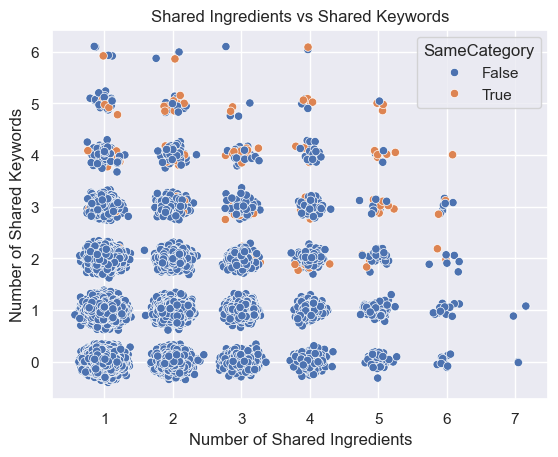
\includegraphics[width=0.7\linewidth]{Report/ReportLatex/Images/Neo4J/plotQuery6.png}
    \caption{Plot Query 6}
    \label{fig:enter-label}
    \end{figure}
    The plot above aims to identify a correlation between recipes that share ingredients or keywords and their belonging to the same category. The parameter used for the query is the recipe "Sesame Chicken With Cream Sauce". Gaussian noise was added to the data to simplify the visualization of distances between recipes in the plot. The plot seems to reveal a correlation: the greater the number of shared keywords and ingredients, the more likely a recipe is to belong to the same category as the given one.
    \clearpage
    \item \addcontentsline{toc}{subsection}{Query 7 - Analyze Recipe Categories by Average Cooking Time and Ingredient Count}
          \textbf{Analyze Recipe Categories by Average Cooking Time and Ingredient Count}\\
    This query is designed to find recipe categories that require the minimum average amount of time.
    Steps:
    \begin{itemize}
        \item Category Information:\\
The query starts by matching Recipe nodes that are related to RecipeCategory nodes through the BELONGS\_TO relationship.
It filters out recipes where the TotalTime is null, ensuring only recipes with a specified total time are considered.
    \item Ingredient Count:\\
The query then matches the Ingredient nodes related to each recipe via the CONTAINS relationship. This allows it to count the number of unique ingredients per recipe.
    \item Aggregation:\\
The total time for each recipe is extracted in minutes (r.TotalTime.minutes AS totalTimeMinutes), and the number of ingredients in each recipe is counted.
    \end{itemize}
The query then calculates the following aggregated values for each category:
    \begin{itemize}
        \item Average total time (avgTotalTimeMinutes): The average total time for all recipes in the category.
        \item Minimum total time (minTotalTimeMinutes): The minimum total time across all recipes in the category.
        \item Maximum total time (maxTotalTimeMinutes): The maximum total time across all recipes in the category.
        \item Average number of ingredients (avgIngredientsPerCategory): The average number of ingredients for recipes in the category.
    \end{itemize}
The query returns the category name (category), the average total time in minutes (avgTotalTimeMinutes), the minimum and maximum total times (minTotalTimeMinutes and maxTotalTimeMinutes), and the average number of ingredients per recipe (avgIngredientsPerCategory).
The results are sorted by the average total time in ascending order, so categories with the least average total time appear first.\\
    \subsubsection{Query}
\begin{CypherQuery}
.
MATCH (r:Recipe)-[:BELONGS_TO]->(c:RecipeCategory)
WHERE r.TotalTime IS NOT NULL
MATCH (r)-[:CONTAINS]->(i:Ingredient)
WITH c, r, r.TotalTime.minutes AS totalTimeMinutes,
COUNT(DISTINCT i) AS numIngredients
WITH c, AVG(totalTimeMinutes) AS avgTotalTimeMinutes,
MIN(totalTimeMinutes) AS minTotalTimeMinutes,
MAX(totalTimeMinutes) AS maxTotalTimeMinutes,
AVG(numIngredients) AS avgIngredientsPerCategory
RETURN c.name AS category,
tointeger(avgTotalTimeMinutes) AS avgTotalTimeMinutes,
tointeger(minTotalTimeMinutes) AS minTotalTimeMinutes,
tointeger(maxTotalTimeMinutes) AS maxTotalTimeMinutes,
tointeger(avgIngredientsPerCategory) AS avgIngredientsPerCategory
ORDER BY avgTotalTimeMinutes ASC;
\end{CypherQuery}
    \subsubsection{Results}
    The following table displays the first 20 lines of the result.
\begin{table}[h!]
\small % Reduce font size
\centering
\setlength{\tabcolsep}{4pt} % Adjust column spacing
\begin{tabular}{p{3cm}p{3cm}p{3cm}p{3cm}p{3cm}}
\toprule
\textbf{category} & \textbf{avgTotalTime Minutes} & \textbf{minTotalTime Minutes} & \textbf{maxTotalTime Minutes} & \textbf{avgIngredients PerCategory} \\
\midrule
"Oatmeal"            & 4  & 4   & 4   & 5 \\
"Szechuan"           & 5  & 5   & 5   & 5 \\
"Smoothies"          & 7  & 2   & 70  & 3 \\
"< 15 Mins"          & 9  & 0   & 15  & 5 \\
"Turkish"            & 10 & 10  & 10  & 6 \\
"Korean"             & 10 & 10  & 10  & 6 \\
"Bath/Beauty"        & 10 & 3   & 20  & 2 \\
"Spanish"            & 11 & 5   & 17  & 8 \\
"Household Cleaner"  & 14 & 2   & 50  & 2 \\
"No Shell Fish"      & 15 & 15  & 15  & 8 \\
"Salad Dressings"    & 15 & 1   & 125 & 7 \\
"Spicy"              & 17 & 5   & 45  & 4 \\
"Whitefish"          & 20 & 20  & 20  & 8 \\
"Melons"             & 20 & 0   & 45  & 6 \\
"Pasta Shells"       & 22 & 0   & 40  & 8 \\
"Microwave"          & 22 & 15  & 35  & 2 \\
"< 30 Mins"          & 23 & 16  & 30  & 6 \\
"Peanut Butter"      & 23 & 10  & 45  & 6 \\
"Vietnamese"         & 23 & 5   & 40  & 9 \\
"Hunan"              & 24 & 24  & 24  & 8 \\
\bottomrule
\end{tabular}
\caption{Analyze Recipe Categories by Average Cooking Time and Ingredient Count.}
\label{tab:category_data}
\end{table}
\subsubsection{Analysis}
\begin{figure}[H]
    \centering
    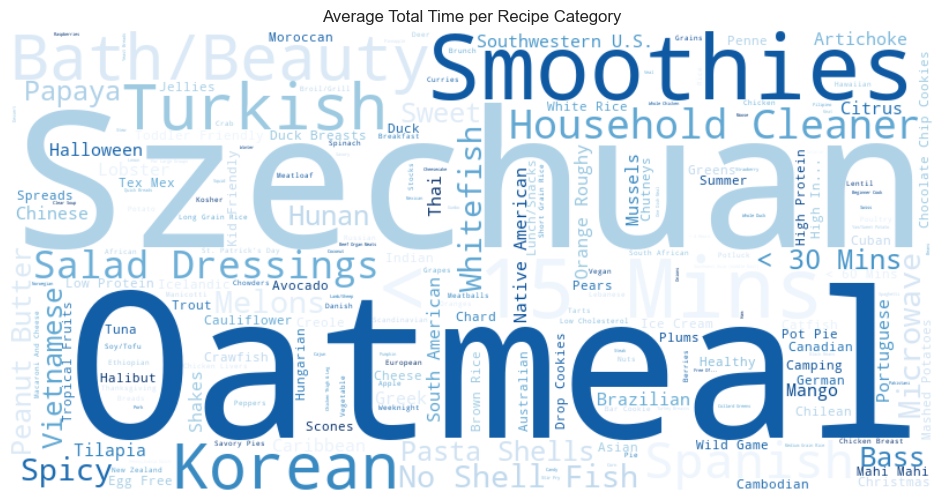
\includegraphics[width=\linewidth]{Report/ReportLatex/Images/Neo4J/plotQuery7.png}
    \caption{Plot Query 7}
    \label{fig:enter-label}
    \end{figure}
The word cloud above highlights the categories of the dataset that require the shortest average preparation time. This visualization can be particularly useful for identifying quick-to-make recipe categories, helping users who are looking for time-efficient cooking options or planning meals on a tight schedule.
    \clearpage
    \item \addcontentsline{toc}{subsection}{Query 8 - Rank Ingredients by Average Recipe Ratings and Popularity}
          \textbf{Rank Ingredients by Average Recipe Ratings and Popularity}\\
    This query identifies the ingredients used in the recipes with the highest ratings and orders them based on a weighted average rating. The weighting is logarithmically scaled by the number of reviews for each ingredient to balance the impact of popularity and rating quality.\\
    Steps:
 \begin{itemize}
     \item MATCH Clause:\\
Retrieves the relationship between ingredients (i), recipes (r), and reviews (review) by navigating through the graph structure.
    \item WITH Clause:\\
Gathers the ingredient name (i.name) as Ingredient, the review rating (review.rating) as Rating, and the entire review node (review) for further computation.
    \item RETURN and ORDER BY Clause:\\
It calculates the average rating for each ingredient (AvgRating) rounded to two decimal places, counts the total number of reviews for each ingredient (ReviewCount) and orders the results by a calculated score: AvgRating * log10(ReviewCount). This formula weights the average rating by the logarithm of the number of reviews, emphasizing ingredients with higher reviews while mitigating the dominance of highly-rated but less-reviewed ingredients.
    \item Output:
The result is a list of ingredients sorted by their significance in recipes with high ratings, where significance is determined by a combination of average rating and review volume. This is useful for identifying the most impactful ingredients in highly regarded recipes.
 \end{itemize}

    \subsubsection{Query}
\begin{CypherQuery}
.
MATCH (i:Ingredient)<-[:CONTAINS]-(r:Recipe)<-[:FOR]-(review:Review)
WITH i.name AS Ingredient,
review.rating AS Rating,review
RETURN Ingredient, round(Avg(Rating), 2) AS AvgRating,
COUNT(review) AS ReviewCount
ORDER BY AvgRating * log10(ReviewCount) DESC;
\end{CypherQuery}
    \subsubsection{Results}
    The following table displays the first 20 lines of the result.
    \begin{table}[h!]
\small % Reduce font size
\centering
\begin{tabularx}{\textwidth}{>{\raggedright\arraybackslash}Xcc}
\toprule
\textbf{Ingredient} & \textbf{AvgRating} & \textbf{ReviewCount} \\
\midrule
"salt"               & 4.41 & 10236 \\
"butter"             & 4.42 & 6492 \\
"sugar"              & 4.41 & 6241 \\
"onion"              & 4.44 & 4226 \\
"flour"              & 4.42 & 4153 \\
"olive oil"          & 4.47 & 3404 \\
"eggs"               & 4.39 & 3923 \\
"water"              & 4.38 & 3774 \\
"milk"               & 4.42 & 3415 \\
"brown sugar"        & 4.49 & 2980 \\
"garlic cloves"      & 4.47 & 2990 \\
"parmesan cheese"    & 4.55 & 2418 \\
"garlic"             & 4.54 & 2253 \\
"baking soda"        & 4.42 & 2610 \\
"vanilla"            & 4.43 & 2559 \\
"pepper"             & 4.41 & 2633 \\
"baking powder"      & 4.36 & 2529 \\
"egg"                & 4.36 & 2446 \\
"lemon juice"        & 4.52 & 1684 \\
"black pepper"       & 4.48 & 1726 \\
\bottomrule
\end{tabularx}
\caption{Rank Ingredients by Average Recipe Ratings and Popularity.}
\label{tab:ingredient_data}
\end{table}

    \clearpage
    \item \addcontentsline{toc}{subsection}{Query 9 - Find Commonly Paired Ingredients, Excluding Disliked Items}
          \textbf{Find Commonly Paired Ingredients, Excluding Disliked Items}\\
    This query identifies pairs of ingredients the user likes that frequently appear together in recipes, excluding any ingredients the user dislikes. The aim is to suggest ingredient combinations that match well and might appeal to the user based on their preferences.
    \begin{itemize}
        \item WITH Clause:\\
Defines a list of ingredients, given to the query as a parameter, that the user dislikes (NotLikedIngredients) to filter them out from the query.
        \item MATCH Clause:\\
Finds pairs of ingredients (i1 and i2) contained in the same recipe (r) through the :CONTAINS relationship.
        \item WHERE Clause:\\
Ensures the query only considers pairs of ingredients where:
i1.name < i2.name: Prevents duplicate pairs and neither ingredient is in the NotLikedIngredients list: excludes undesired ingredients from the analysis.
        \item WITH Clause:\\
Groups data by ingredient pairs and the recipes in which they co-occur.
        \item RETURN Clause:\\
Returns the names of the paired ingredients (Ingredient1 and Ingredient2) and calculates the number of distinct recipes where each pair appears together (CoOccurrenceCount).
        \item ORDER BY Clause:\\
Sorts the results by the number of co-occurrences in descending order, prioritizing the most frequent ingredient pairs.
        \item Output:\\
The query produces a ranked list of ingredient pairs that the user is likely to enjoy and that frequently appear together in recipes. \\This information can help generate suggestions for ingredient combinations that match well, potentially inspiring new recipes or meal ideas aligned with the user's preferences.
    \end{itemize}
    \subsubsection{Query}
\begin{CypherQuery}
.
WITH \$ingredients AS NotLikedIngredients
MATCH
(i1:Ingredient)<-[:CONTAINS]-(r:Recipe)-[:CONTAINS]->(i2:Ingredient)
WHERE i1.name < i2.name 
AND NOT i1.name  IN NotLikedIngredients 
AND NOT i2.name IN NotLikedIngredients
WITH i1, i2, r
RETURN i1.name AS Ingredient1,
i2.name AS Ingredient2,
COUNT(DISTINCT r) AS CoOccurrenceCount
ORDER BY CoOccurrenceCount DESC;
\end{CypherQuery}
    \subsubsection{Results}
    The results change based on what ingredients that the user don't like are put as a parameter. In this table the parameter  \$ingredients is set as the list 
\begin{CypherQuery}
.
['fish','broccoli','potato']
\end{CypherQuery}
    The table shows the first 20 lines of the results.
    \begin{table}[h!]
\small % Reduce font size
\centering
\begin{tabularx}{\textwidth}{>{\raggedright\arraybackslash}X>{\raggedright\arraybackslash}Xc}
\toprule
\textbf{Ingredient1} & \textbf{Ingredient2} & \textbf{CoOccurrenceCount} \\
\midrule
"butter"            & "salt"              & 1031 \\
"salt"              & "sugar"             & 959  \\
"eggs"              & "salt"              & 800  \\
"pepper"            & "salt"              & 715  \\
"flour"             & "salt"              & 679  \\
"onion"             & "salt"              & 645  \\
"butter"            & "eggs"              & 637  \\
"salt"              & "water"             & 635  \\
"butter"            & "sugar"             & 616  \\
"butter"            & "flour"             & 572  \\
"eggs"              & "sugar"             & 570  \\
"olive oil"         & "salt"              & 551  \\
"baking powder"     & "salt"              & 524  \\
"milk"              & "salt"              & 509  \\
"all-purpose flour" & "salt"              & 484  \\
"flour"             & "sugar"             & 472  \\
"butter"            & "milk"              & 459  \\
"baking soda"       & "salt"              & 453  \\
"garlic cloves"     & "olive oil"         & 427  \\
"garlic cloves"     & "salt"              & 414  \\

\bottomrule
\end{tabularx}
\caption{Find Commonly Paired Ingredients, Excluding Disliked Items.}
\label{tab:cooccurrence_data}
\end{table}

    \clearpage
    \item \addcontentsline{toc}{subsection}{Query 10 - Discover High-Protein Low-Calorie Recipes with Top Ratings and specific ingredients}
          \textbf{Discover High-Protein Low-Calorie Recipes with Top Ratings and specific ingredients}\\
    This query is designed to find diet-friendly recipes that meet the following criteria:
    \begin{itemize}
        \item Ingredient Inclusion: The recipe must contain specific ingredients, given to the query as a parameter
        \item Calorie Restriction: The recipe must have a total calorie count of 500 or less.
        \item  High Protein and Low Fat:
The query calculates the protein ratio, carbohydrate ratio, and fat ratio for each recipe by dividing the respective macronutrient content by the total calories.
It then prioritizes recipes with the highest protein-to-fat efficiency, using the formula ProteinRatio/FatRatio for ranking.
        \item Positive Reviews: The recipe must have an average review rating of 4.0 or higher.
    \end{itemize}
The query outputs the following details for each recipe that matches the criteria:
\begin{itemize}
    \item RecipeName: The name of the recipe.
    \item AvgRating: The average review score for the recipe.
    \item ProteinRatio: The ratio of protein to total calories (rounded to two decimal places).
    \item CarboRatio: The ratio of carbohydrates to total calories (rounded to two decimal places).
    \item FatRatio: The ratio of fat to total calories (rounded to two decimal places).
\end{itemize}
Recipes are sorted at the end by the highest protein-to-fat efficiency in descending order, ensuring that recipes with the best protein-to-fat balance are prioritized.
This query is particularly useful for users seeking healthy recipes that:
\begin{itemize}
    \item Contain specific ingredients.
    \item Stay within calorie limits.
    \item Maximize protein intake while minimizing fat content.
    \item Have been rated highly by other users.
\end{itemize}
    \subsubsection{Query}
\begin{CypherQuery}
.
MATCH (recipe:Recipe)-[:CONTAINS]->(ingredient:Ingredient)
MATCH (recipe)<-[:FOR]-(review:Review)
WHERE ingredient.name IN \$ingredients 
AND recipe.Calories <= 500
WITH recipe, 
round(recipe.ProteinContent / recipe.Calories,2) AS protein_ratio,
round(recipe.CarbohydrateContent / recipe.Calories,2) AS carbo_ratio,
round(recipe.FatContent / recipe.Calories,2) AS fat_ratio,
avg(review.rating) AS avg_review_rating
WHERE avg_review_rating >= 4
RETURN recipe.Name AS RecipeName, 
avg_review_rating AS AvgRating, 
protein_ratio AS ProteinRatio, 
carbo_ratio AS CarboRatio, 
fat_ratio AS FatRatio
ORDER BY ProteinRatio/FatRatio DESC;
\end{CypherQuery}

    \subsubsection{Results}
    The results change based on what list of ingredients is put as a parameter. In this table
the parameter \$recipeName is set as 
\begin{CypherQuery}
.
['chicken', 'spinach']
\end{CypherQuery}
The table shows the first 20 lines of results.
    \begin{table}[h!]
\small % Reduce font size
\centering
\begin{tabularx}{\textwidth}{>{\raggedright\arraybackslash}Xcccc}
\toprule
\textbf{RecipeName} & \textbf{AvgRating} & \textbf{ProteinRatio} & \textbf{CarboRatio} & \textbf{FatRatio} \\
\midrule
"Spinach Coriander Soup"                            & 4.0  & 0.05 & 0.21 & 0.01 \\
"Chicken Noodle Soup"                               & 5.0  & 0.05 & 0.17 & 0.02 \\
"Banana Berry Blast Green Smoothie"                & 5.0  & 0.02 & 0.25 & 0.01 \\
"Spinach and Feta Crepes"                           & 5.0  & 0.06 & 0.11 & 0.04 \\
"Chicken Etc. Risotto"                              & 5.0  & 0.04 & 0.10 & 0.03 \\
"Pizza With Pizzazz"                                & 5.0  & 0.04 & 0.15 & 0.03 \\
"Country Dijon Poulet"                              & 5.0  & 0.06 & 0.05 & 0.05 \\
"Chicken-Vegetable Casserole"                       & 5.0  & 0.06 & 0.07 & 0.06 \\
"Hidden Valley Four Cheese Pasta Bake With Spinach and Bacon \#RSC" & 5.0  & 0.04 & 0.12 & 0.04 \\
"Chicken Jardiniere Au Vermouth"                   & 4.0  & 0.07 & 0.02 & 0.07 \\
"Pumpkin and Spinach Pizza"                         & 5.0  & 0.06 & 0.08 & 0.06 \\
"E-Z Roast Chicken"                                & 4.85 & 0.07 & 0.01 & 0.08 \\
"Chicken With Vinegar (Mark Bittman)"              & 5.0  & 0.07 & 0.00 & 0.08 \\
"Lemon, Beet and Fennel Roast Chicken"             & 5.0  & 0.06 & 0.03 & 0.07 \\
"Korean Japchae - a Beef and Vegetable Glass Noodle Stir-Fry" & 5.0  & 0.05 & 0.06 & 0.06 \\
"Comfort Food Rice Casserole"                       & 5.0  & 0.04 & 0.11 & 0.05 \\
"Quinoa Stuffing With Leeks, Walnuts and Cherries" & 5.0  & 0.03 & 0.14 & 0.04 \\
"Fast Chicken Enchiladas"                           & 4.5  & 0.03 & 0.13 & 0.04 \\
"Creamy Spinach and Avocado Pasta"                 & 5.0  & 0.03 & 0.15 & 0.04 \\
"Hot Chicken Salad"                                & 5.0  & 0.05 & 0.05 & 0.07 \\

\bottomrule
\end{tabularx}
\caption{Discover High-Protein Low-Calorie Recipes with Top Ratings and specific ingredients.}
\label{tab:recipe_data}
\end{table}

\end{enumerate}
\clearpage
\section{Elasticsearch}

\subsection{Queries}\label{sec:ElastisearchQueries}
\begin{enumerate}
    \item \addcontentsline{toc}{subsection}{Query 1 - Recipes for a romantic dinner}
          \textbf{Recipes for a romantic dinner}

    This search query, that targets recipes with a specific number of servings and prioritizes those explicitly associated with romance, was designed to identify recipes suitable for a romantic dinner. 
    The query is structured as a compound query: firstly, it performes a must query, which makes sure that the RecipeServings field has a value between 2 and 3. This range corresponds to a meal for two people, accommodating varying portion sizes depending on individual appetites.
    In addition to this, a should clause is added to boost the relevance of recipes that are specifically associated with romantic themes. The boosting mechanism ensures that recipes explicitly labeled or described as romantic are ranked higher in the search results. The should clause includes the following conditions:
    
    Reviews: Recipes receive a boost if the word "romantic" appears in any of their reviews. This is achieved through a nested query that navigates into the Reviews object and matches the Review field for the term "romantic." This captures user feedback or sentiments indicating that the recipe has been perceived as good for romantic occasions.

    Keywords: Recipes are boosted if the Keywords field contains the term "romantic." This field often contains tags or descriptive phrases added by the recipe creator, providing a direct indication of the intended use of the recipe.

    Description: Recipes with the term "romantic" in the Description field are also given a higher ranking. This ensures that recipes designed for romantic occasions, as described by the author, are prioritized in the results.

    Aggregated Rating: To ensure quality, recipes with an AggregatedRating of 3.5 or higher receive additional weighting. However, a boost was not applied to this query, as it is considered less critical than the others for the purpose of this search.

    \subsubsection{Query}
    \begin{lstlisting}[language=Elasticsearch]
    
GET /recipesandreviews/_search
{
  "query": {
    "bool": {
      "must": [
        {
          "range": {
            "RecipeServings": {
              "gte": 2,
              "lte": 3
            }}}],
      "should": [
        {
          "nested": {
            "path": "Reviews",
            "query": {
              "match": {
                "Reviews.Review": {
                  "query": "romantic",
                  "boost": 2
                }}}}},
        {
          "match": {
            "Keywords": {
              "query": "romantic",
              "boost": 2
            }}},
        {
          "match": {
            "Description": {
              "query": "romantic",
              "boost": 2
            }}},
        {
          "range": {
            "AggregatedRating": {
              "gte": 3.5
            }}}]}}}

    \end{lstlisting}
    \subsubsection{Result}
    Here, the beginning of the first two output documents returned by the query is shown.
    \begin{figure}[H]
    \centering
    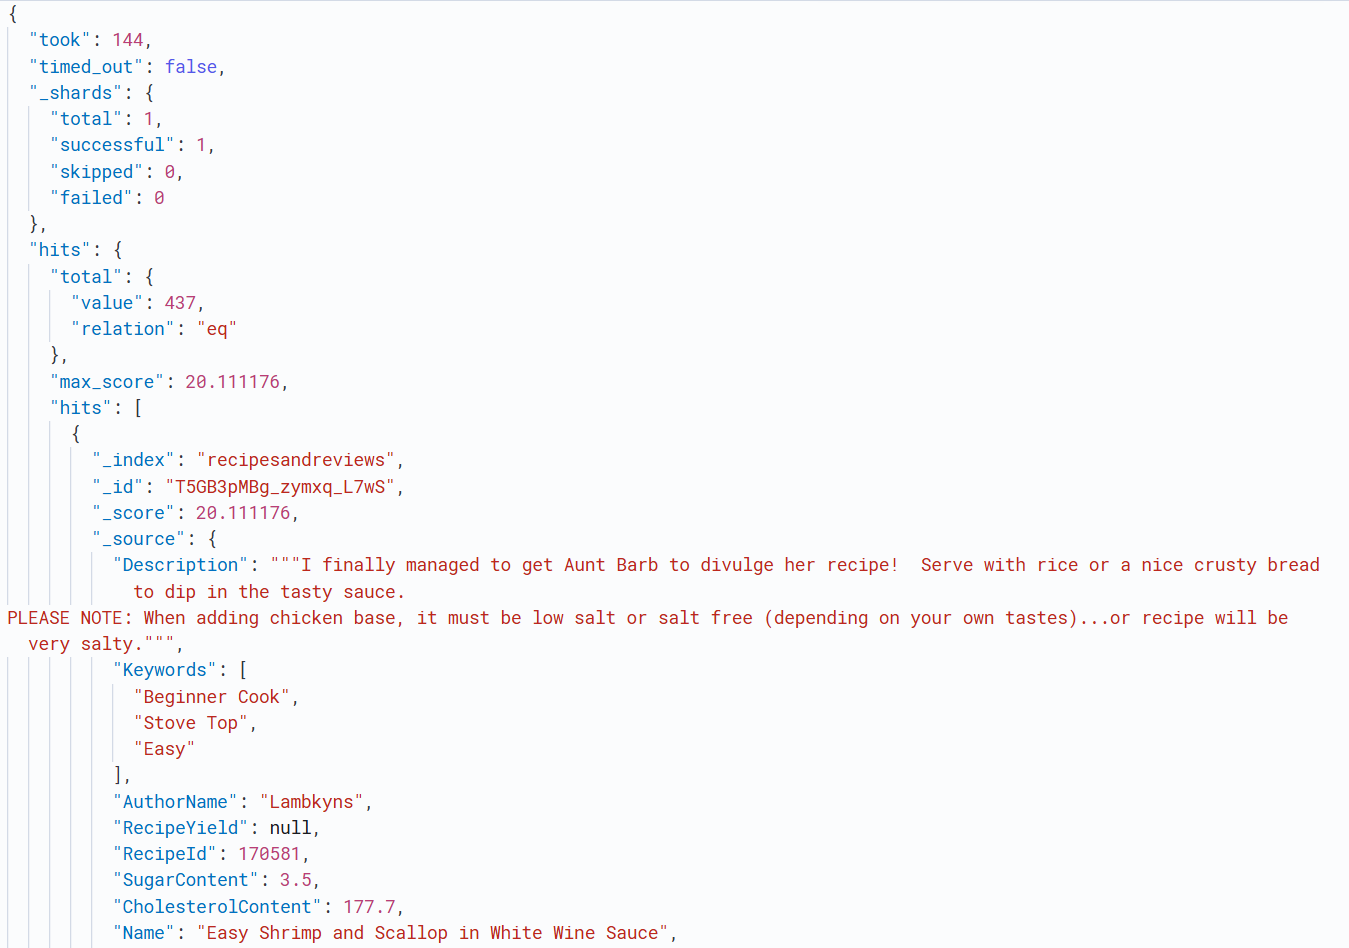
\includegraphics[width=0.8\linewidth]{Report/ReportLatex/Images/ElasticsearchResults/RomanticDinner1.png}
    \caption{1st result}
    \label{fig:enter-label}
    \end{figure}
    \begin{figure}[H]
    \centering
    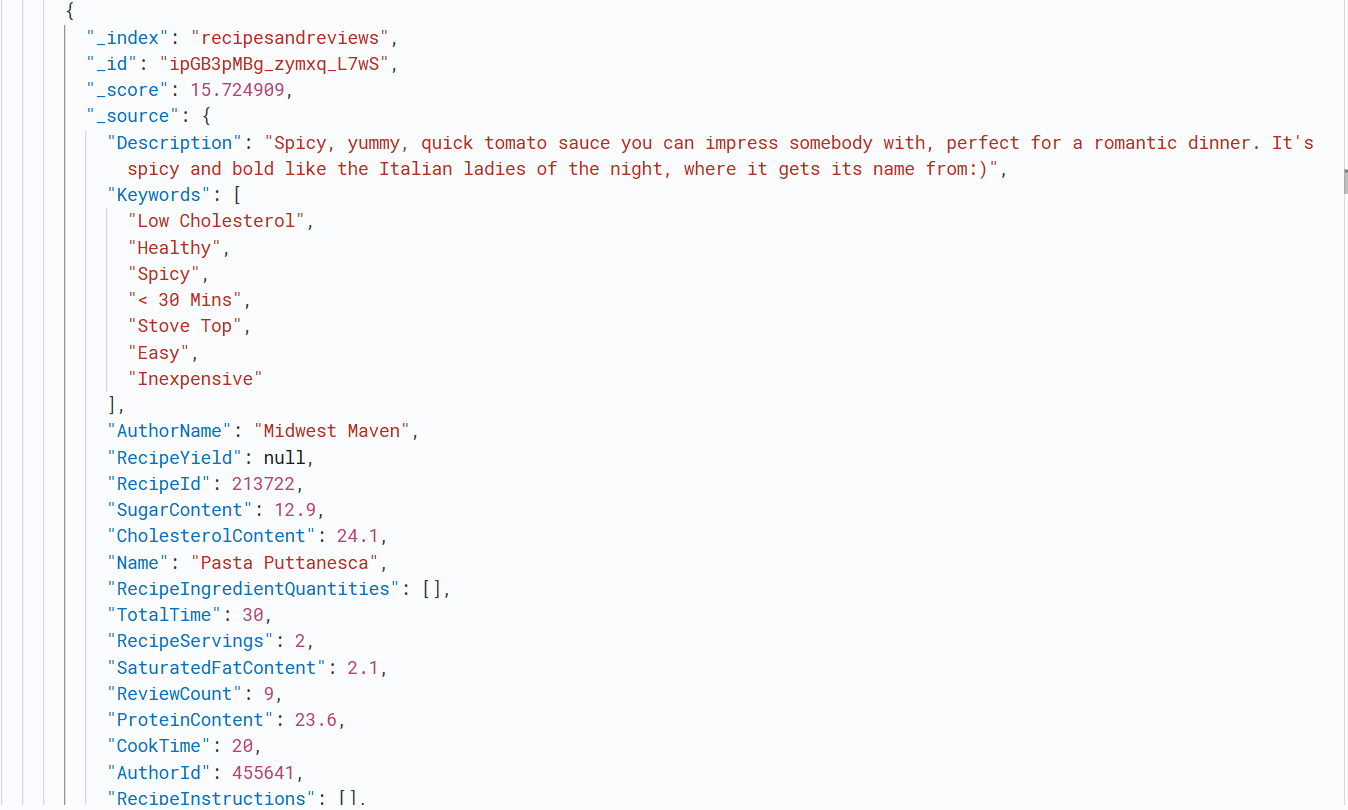
\includegraphics[width=0.9\linewidth]{Report/ReportLatex/Images/ElasticsearchResults/RomanticDinner2.png}
    \caption{2nd result}
    \label{fig:enter-label}
    \end{figure}
    \clearpage
    
    \item \addcontentsline{toc}{subsection}{Query 2 - Recipes made only using a microwave}
          \textbf{Recipes made only using a microwave }

    This query is designed to help a student who only has a microwave and no other appliances find recipes that can be made exclusively with a microwave.
    
    In the must clause, it is ensured that the RecipeInstructions field contains the word "microwave", confirming that the recipe involves using the microwave for cooking. To refine the search further, a must\_not clause was added to exclude recipes mentioning the use of other appliances, such as an oven, pan, pot, or fryer, in the Keywords or RecipeInstructions fields. This ensures that the results include only recipes that rely exclusively on the microwave.

    Additionally, the should clause is used to assign a higher score to recipes that emphasize the microwave as a key element. The term "microwave" is searched for in both the Keywords and the Reviews.Review field, as its presence in these areas indicates that the microwave is considered an important part of the recipe, either by the recipe creator or reviewers.

    This approach ensures that students will find recipes specifically designed for microwave use, without the need for additional cooking appliances, and gives extra weight to those that emphasize the microwave's role in the cooking process. A minimum should match was not set, as the fundamental parameters for this query are defined solely by the conditions in the must and must not clauses.

    \subsubsection{Query}
    \begin{lstlisting}[language=Elasticsearch]
GET /recipesandreviews/_search
{
  "query": {
    "bool": {
      "must": [
        {
          "match": {
            "RecipeInstructions": "microwave"
          }}],
      "must_not": [
        {
          "match": {
            "Keywords": {
              "query": "oven pan pot fryer",
              "operator": "or"
            }}},
        {
          "match": {
            "RecipeInstructions": {
              "query": "oven pan pot fryer",
              "operator": "or"
            }}}],
      "should": [
        {
          "match": {
            "Keywords": "microwave"
          }},
        {
          "nested": {
            "path": "Reviews",
            "query": {
              "match": {
                "Reviews.Review": "microwave"
              }}}}]}}}
    \end{lstlisting}

    \subsubsection{Result}
    Here is shown the beginning of the first 2 output documents given by the query. 
    \begin{figure}[H]
    \centering
    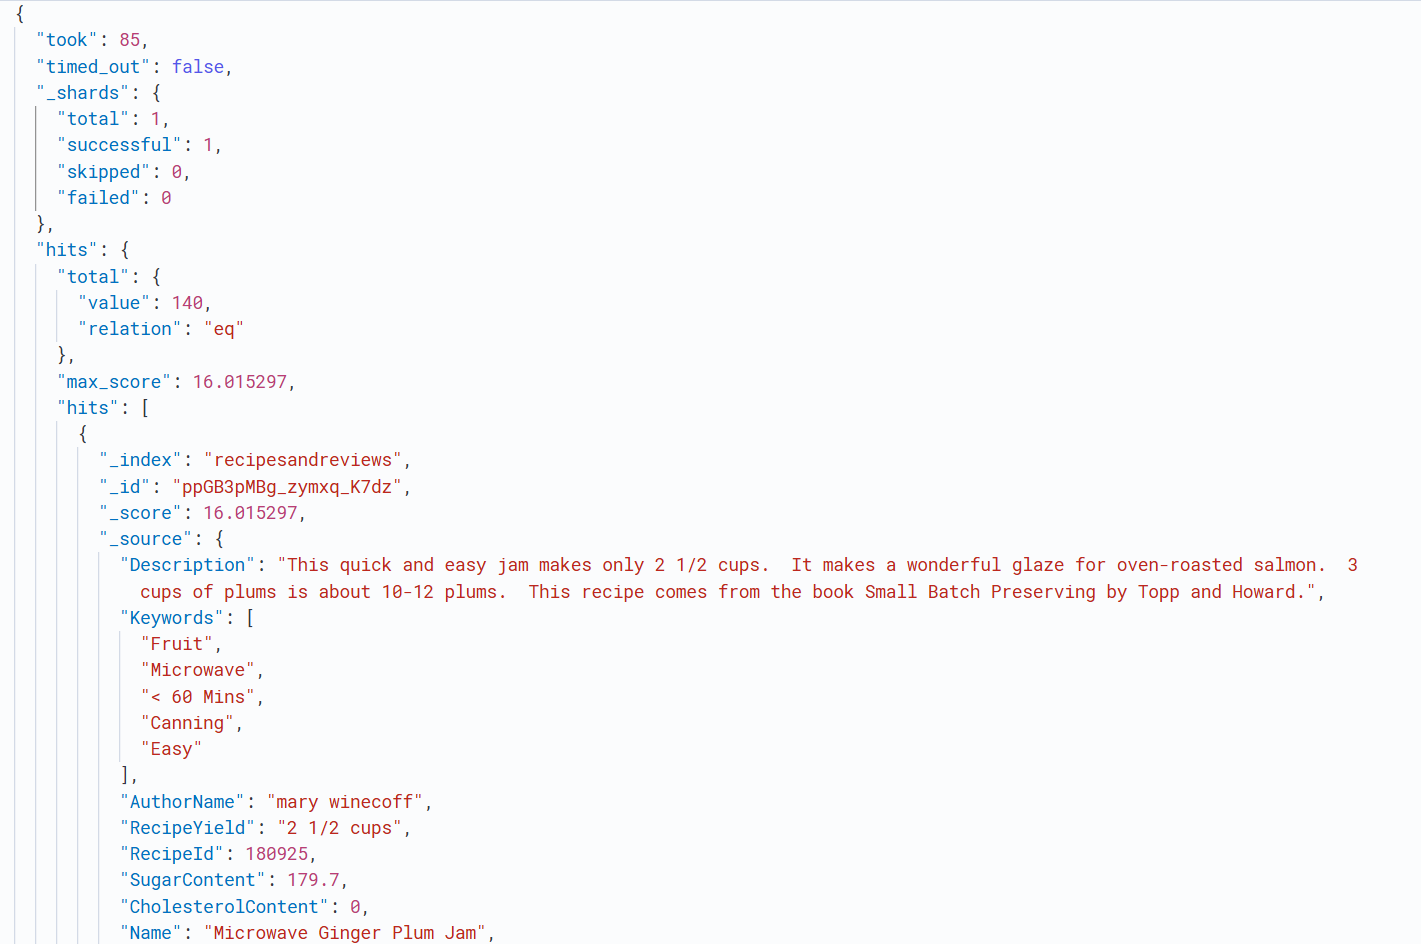
\includegraphics[width=0.8\linewidth]{Report/ReportLatex/Images/ElasticsearchResults/microwave1.png}
    \caption{1st result}
    \label{fig:enter-label}
    \end{figure}
    \begin{figure}[H]
    \centering
    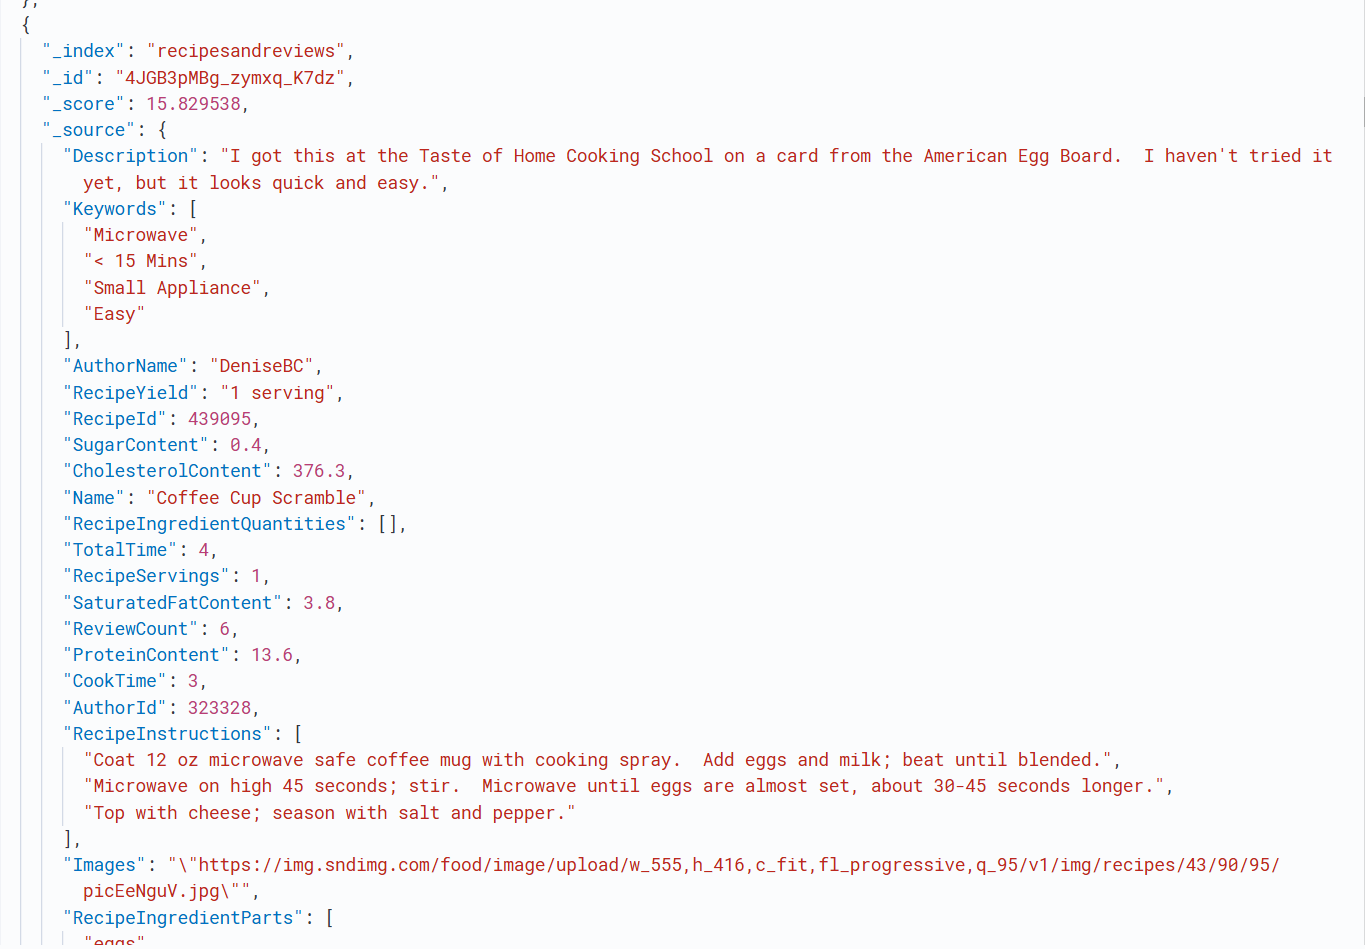
\includegraphics[width=0.9\linewidth]{Report/ReportLatex/Images/ElasticsearchResults/microwave2.png}
    \caption{2nd result}
    \label{fig:enter-label}
    \end{figure}
    \clearpage
    
    \item \addcontentsline{toc}{subsection}{Query 3 - Quick Recipes Using All Given Ingredients}
          \textbf{Quick Recipes Using All Given Ingredients}

    This query was designed to find recipes that use all the ingredients provided by a user. To achieve this,  it is employed a must clause that contains a match query and a range query. 
    
    The match query searches for the specified ingredients within the RecipeIngredientParts field (a text field). To ensure all ingredients are included, the match query uses an and operator, meaning only recipes that contain all the listed ingredients will be returned.
    
    The range query filters recipes to include only those with a total time of 30 minutes or less, fulfilling the requirement for quick recipes.
    \subsubsection{Query}
    \begin{lstlisting}[language=Elasticsearch]
GET /recipesandreviews/_search
{
  "query": {
    "bool": {
      "must": [
        {
          "match": {
            "RecipeIngredientParts": {
              "query": "chicken onion cheese",
              "operator": "and"
            }}},
        {
          "range": {
            "TotalTime": {
              "lte": 30
            }}}]}}}
    \end{lstlisting}

    \subsubsection{Result}
    Here is presented the beginning of the output including the metadata, and several images displaying the RecipeIngredientParts field from various recipes, to show the accuracy of the results.
    \begin{figure}[H]
    \centering
    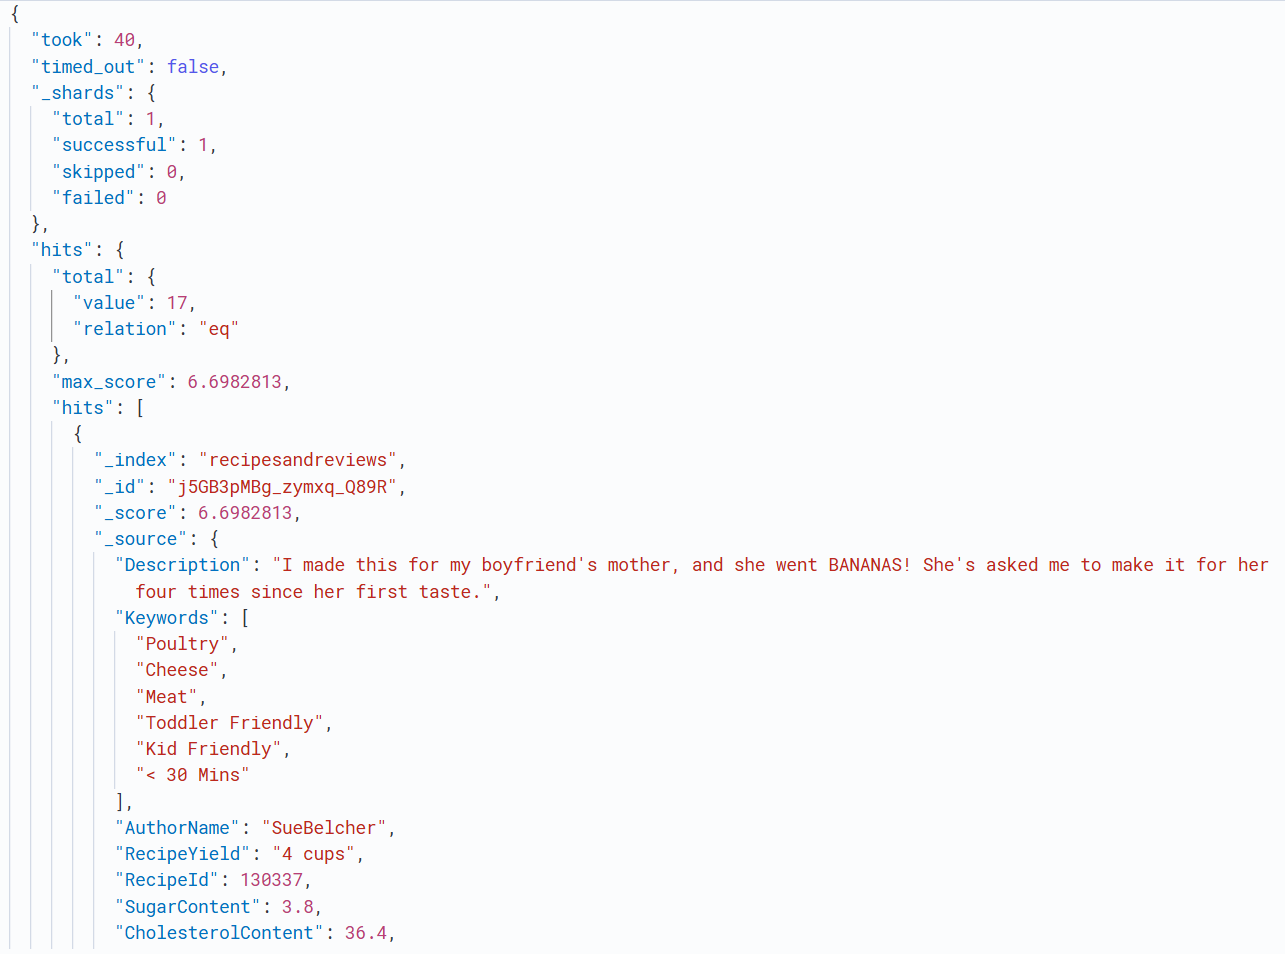
\includegraphics[width=0.9\linewidth]{Report/ReportLatex/Images/ElasticsearchResults/ingredients1.png}
    \caption{1st result}
    \label{fig:enter-label}
    \end{figure}

    \begin{figure}[h!]
    \centering
    \begin{minipage}{0.25\textwidth}
        \centering
        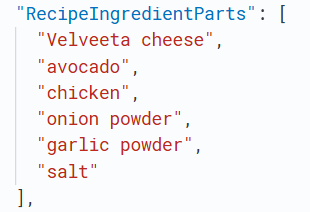
\includegraphics[width=\textwidth]{Report/ReportLatex/Images/ElasticsearchResults/ingredients2.png}
    \end{minipage}%
    \hspace{0.05\textwidth}
    \begin{minipage}{0.25\textwidth}
        \centering
        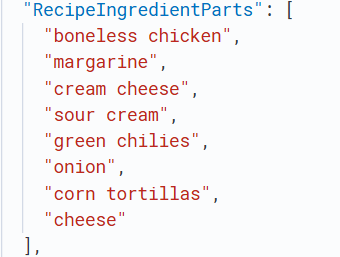
\includegraphics[width=\textwidth]{Report/ReportLatex/Images/ElasticsearchResults/ingredients3.png}
    \end{minipage}%
    \hspace{0.05\textwidth}
    \begin{minipage}{0.25\textwidth}
        \centering
        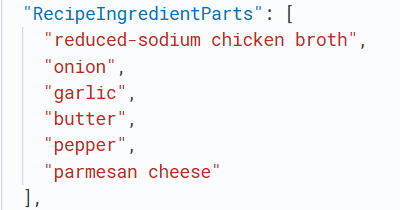
\includegraphics[width=\textwidth]{Report/ReportLatex/Images/ElasticsearchResults/ingredients4.png}
    \end{minipage}
    
    \caption{RecipeIngredientParts}
    \end{figure}
    \clearpage
    
    \item \addcontentsline{toc}{subsection}{Query 4 - Recipes for a party with a lot of servings}
          \textbf{Recipes for a party with a lot of servings}
    
    To identify recipes suitable for hosting a party, the focus was placed on those serving a larger number of people. In the "must" clause, it was specified that the recipes should have a RecipeServings value greater than or equal to 10, ensuring they are suitable for a gathering. Additionally, a "should" clause was applied to give extra weight to recipes that explicitly reference terms related to parties and large events, such as "party" "large groups" "gathering" "celebration" "buffet".

    The should clause includes several fields where these keywords might appear, for example, the Keywords field is searched for terms like "party" and "celebration" with a boost of 2, emphasizing recipes designed with these themes in mind. The RecipeCategory field is also considered, with a boost of 1.5 for categories such as "Party", "Buffet", and "Appetizer", since these are often associated with party-friendly meals. Similarly, the Description field is searched for party-related terms with a boost of 1.5 to highlight recipes that mention large gatherings or events.
    Lastly, the Reviews field was included, with a specific focus on searching within the nested Reviews.Review subfield for mentions of party-related terms. These reviews are boosted with a higher weight (boost of 3)  since in this context the reviews are the most important parameter to account for.
    The minimum\_should\_match parameter is set to 1, ensuring that at least one of the should conditions is to be satisfied for a recipe to be returned in the results

    \subsubsection{Query}
    \begin{lstlisting}[language=Elasticsearch]
GET /recipesandreviews/_search
{
  "query": {
    "bool": {
      "must": [
        {
          "range": {
            "RecipeServings": {
              "gte": 10
            }}}],
      "should": [
        {
          "match": {
            "Keywords": {
              "query": "party, large groups, gathering, celebration, 
              event, buffet",
              "operator": "or",
              "boost": 2
            }}},
        {
          "match": {
            "RecipeCategory": {
              "query": "Dessert, Appetizer, Main, Party, Buffet",
              "operator": "or",
              "boost": 1.5
            }}},
        {
          "match": {
            "Description": {
              "query": "party, large groups, gathering, celebration, event",
              "operator": "or",
              "boost": 1.5
            }}},
        {
          "nested": {
            "path": "Reviews",
            "query": {
              "match": {
                "Reviews.Review": {
                  "query": "party, celebration, gathering, event, buffet",
                  "operator": "or",
                  "boost": 3
                }}}}}],
      "minimum_should_match": 1
    }}}
    \end{lstlisting}

    \subsubsection{Result}
    The first image displays the first result along with the prior metadata. The second image shows some of the reviews in the output, demonstrating that the query successfully retrieved relevant recipes.
    \begin{figure}[H]
    \centering
    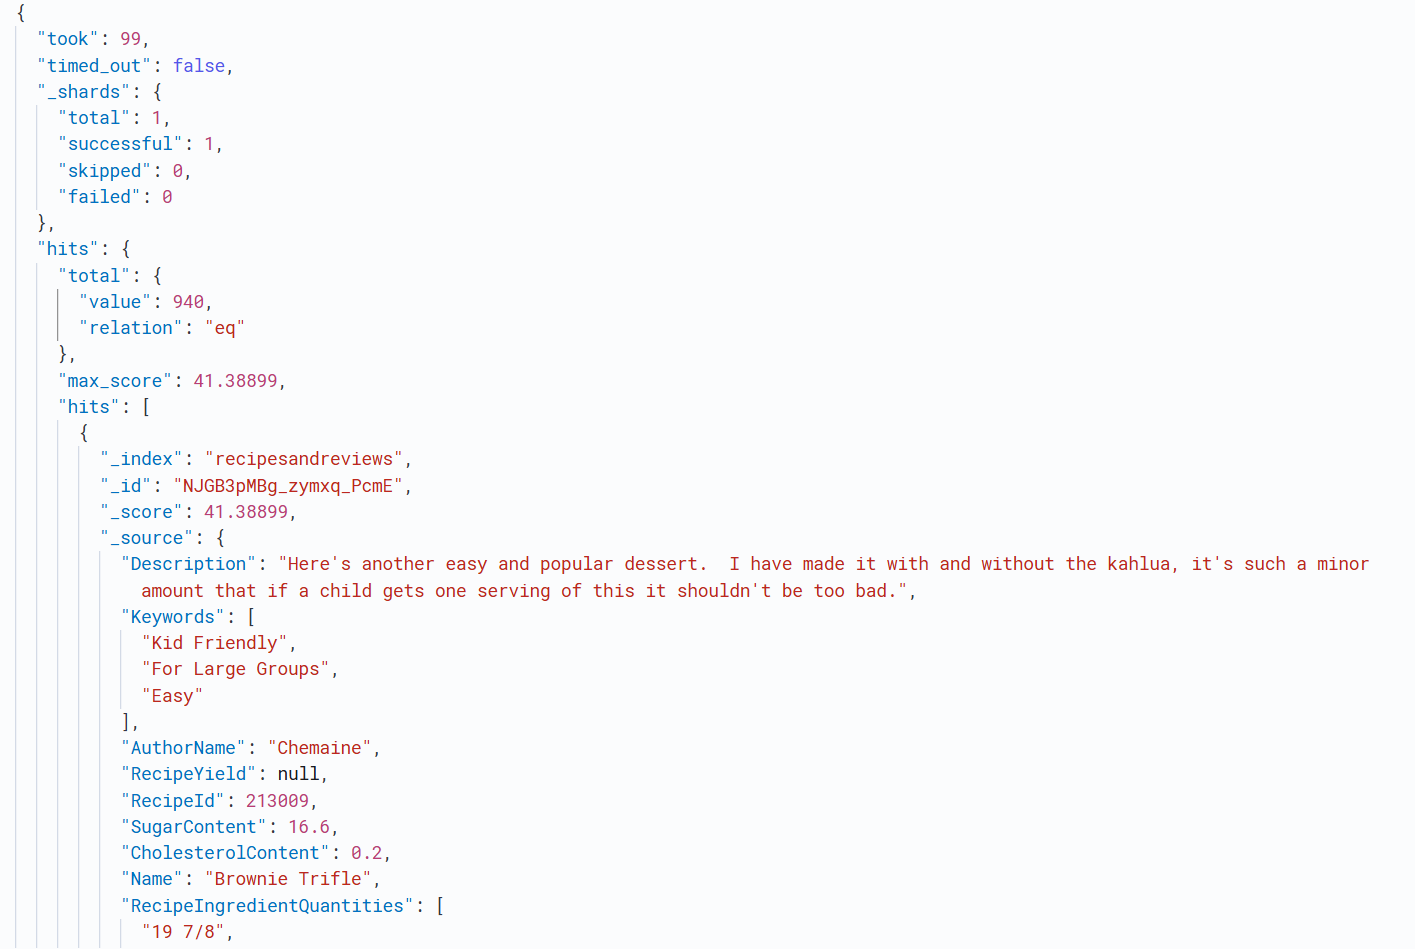
\includegraphics[width=0.9\linewidth]{Report/ReportLatex/Images/ElasticsearchResults/party1.png}
    \caption{1st result}
    \label{fig:enter-label}
    \end{figure}
    \begin{figure}[H]
    \centering
    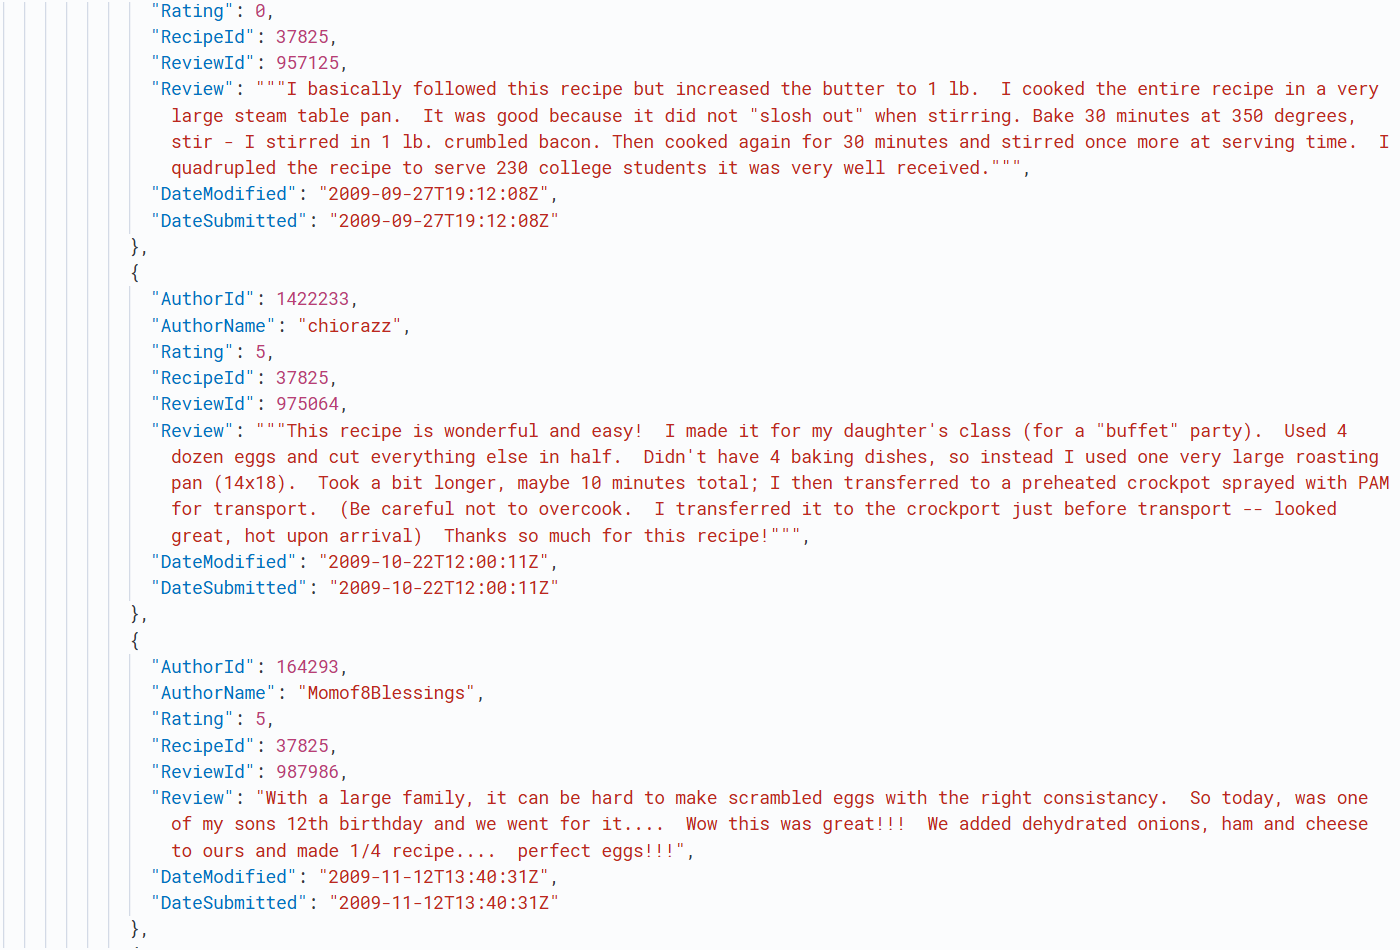
\includegraphics[width=0.9\linewidth]{Report/ReportLatex/Images/ElasticsearchResults/party2.png}
    \caption{Relevant Reviews}
    \label{fig:enter-label}
    \end{figure}
    \clearpage
    
    \item \addcontentsline{toc}{subsection}{Query 5 - Recipes with the best protein/calorie ratio}
          \textbf{Recipes with the best protein/calorie ratio}

    This Elasticsearch query identifies recipes that are high in protein relative to their calorie content, and associated with keywords related to health, fitness, and nutrition. It combines a script-based filter with a relevance scoring system to prioritize results that align with the criteria in the should clause.

    The script filters recipes by calculating the protein to/calorie ratio dynamically. It includes recipes where calories are non-zero, and protein makes up at least 20\% of the total calories. This approach avoids the need to precompute and store the ratio as a separate field, offering flexibility to adapt the logic without re-indexing. 

    The query also ranks recipes higher if they match specific health-related keywords in their description, keywords, recipe category, or user reviews. Words like "healthy", "gym", "protein", "fit" and "nutritious" are used to search for this concept in the data.

    \subsubsection{Query}
    \begin{lstlisting}[language=Elasticsearch]
GET /recipesandreviews/_search
{
  "query": {
    "bool": {
      "filter": [
        {
          "script": {
            "script": {
              "source": """
                if (doc['Calories'].size() > 0 && doc['Calories'].value!= 0) {
                  return doc['ProteinContent'].value / doc['Calories'].value >= 0.2;
                } else {
                  return false;
                }
              """
            }}}],
      "should": [
        {
          "match": {
            "Description": {
              "query": "healthy gym protein fit strong weight nutritious",
              "operator": "or"
              }}},
        {
          "match": {
            "Keywords": {
              "query": "healthy gym protein fit strong weight nutritious",
              "operator": "or",
              "boost": 3
              }}},
        {
          "match": {
            "RecipeCategory": {
              "query": "healthy gym protein fit strong weight nutritious",
              "operator": "or"
              }}},
        {
          "nested": {
            "path": "Reviews",
              "query": {
                "match": {
                  "Reviews.Review": {
                    "query": "healthy gym protein fit strong weight nutritious",
                    "operator": "or"
                    }}}}}]}}}
    \end{lstlisting}

    \subsubsection{Result}
    Here are the beginning portions of the first two output documents returned by the query.
    \begin{figure}[H]
    \centering
    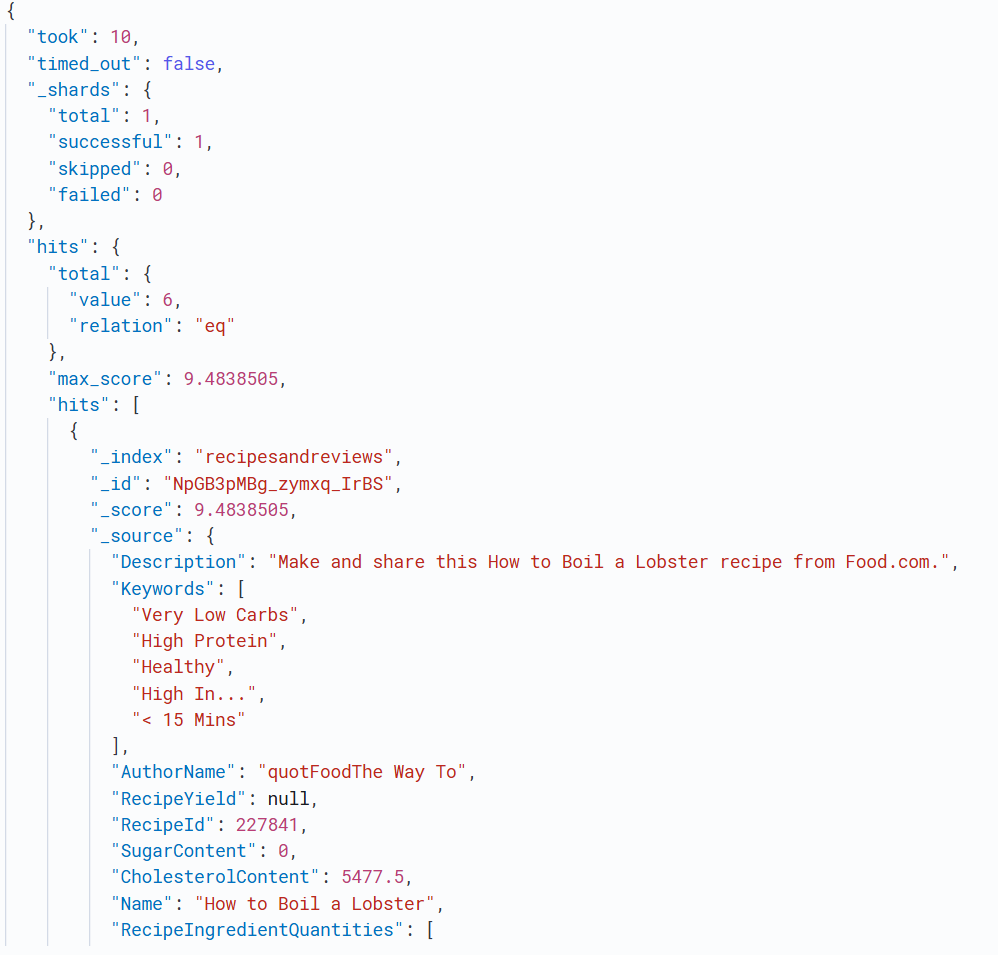
\includegraphics[width=0.8\linewidth]{Report/ReportLatex/Images/ElasticsearchResults/proteins1.png}
    \caption{1st result}
    \label{fig:enter-label}
    \end{figure}
    \begin{figure}[H]
    \centering
    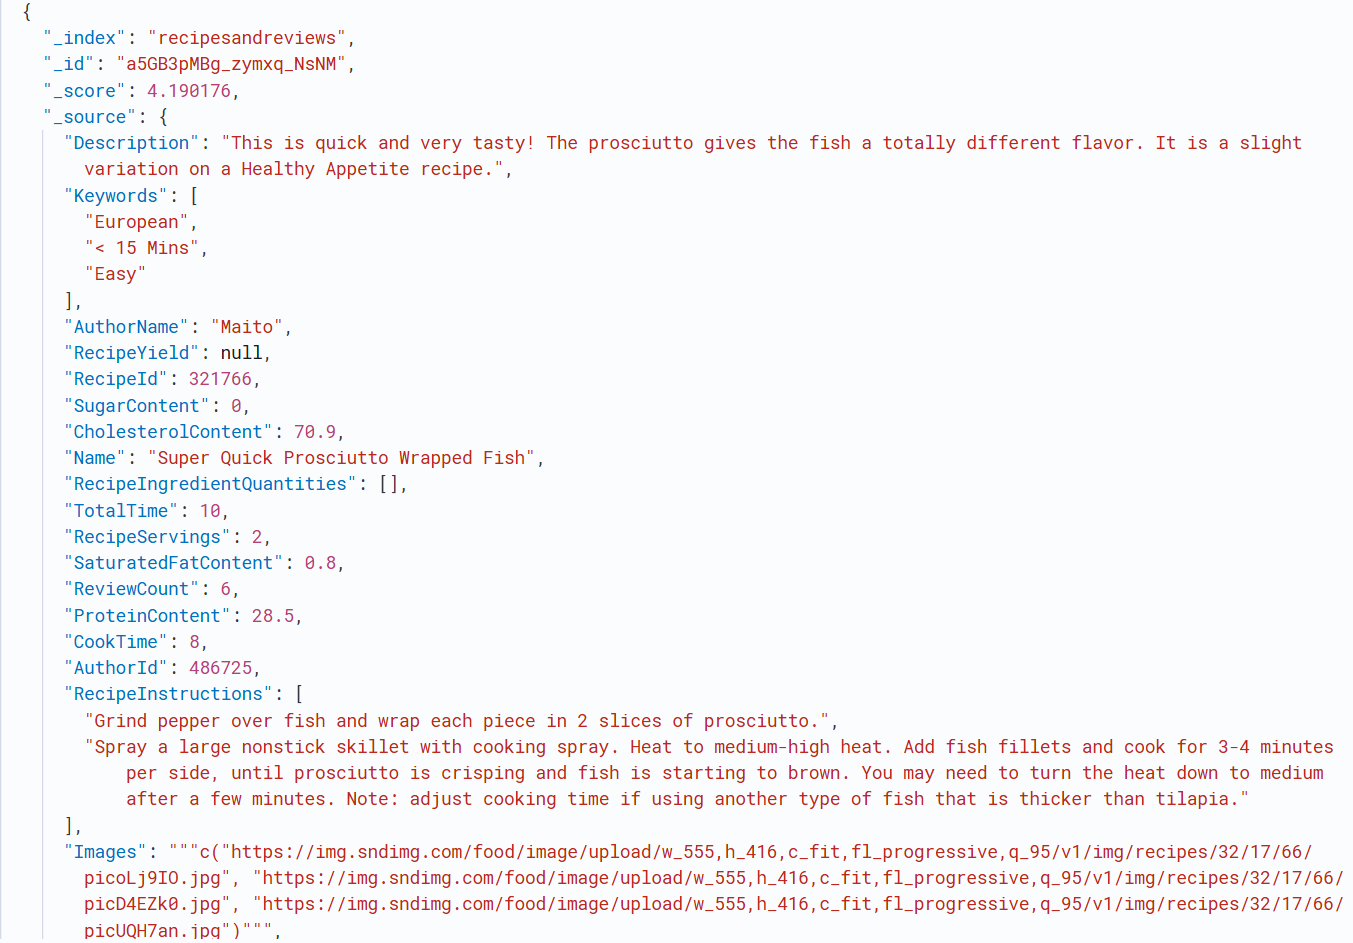
\includegraphics[width=0.8\linewidth]{Report/ReportLatex/Images/ElasticsearchResults/proteins2.png}
    \caption{2nd result}
    \label{fig:enter-label}
    \end{figure}
    
    \clearpage
    
    \item \addcontentsline{toc}{subsection}{Query 6 - Recipes for specific dietary restrictions (lactose intolerance)}
          \textbf{Recipes for specific dietary restrictions (lactose intolerance)}

    This query is designed to find recipes suitable for individuals with lactose intolerance or those following a lactose-free diet. The search first excludes any recipes containing common sources of lactose, such as milk, cheese, lactose, and yogurt, using the must\_not clause. This ensures that recipes with these ingredients are filtered out, as they are not appropriate for people who need to avoid lactose.

    In addition to filtering out lactose-containing ingredients, the query uses a should clause to boost the relevance of recipes that explicitly mention being lactose-free or suitable for those with lactose intolerance. It looks for these terms in the Keywords, Description, and RecipeCategory fields, as well as in Reviews. The query searches for terms like "lactose free" and "lactose intolerant" across these fields to give higher scores to recipes that are clearly labeled as suitable for those with lactose restrictions. This helps prioritize lactose-free recipes, making it easier for users to find meals that meet their dietary needs.

    \subsubsection{Query}
    \begin{lstlisting}[language=Elasticsearch]
GET /recipesandreviews/_search
{
  "query": {
    "bool": {
      "must_not": [
        {
          "match": {
            "RecipeIngredientParts": {
              "query": "milk cheese lactose yogurt",
              "operator": "or"
            }}}],
      "should": [
        {
          "match": {
            "Keywords": "lactose free"
          }},
        {
          "match": {
            "Description": "lactose free intolerant"
          }},
        {
          "match": {
            "RecipeCategory": "lactose free"
          }},
        {
          "nested": {
            "path": "Reviews",
            "query": {
              "match": {
                "Reviews.Review": "lactose free intolerant"
              }}}}]}}}
    \end{lstlisting}

    \subsubsection{Result}
    The beginning of the first and the second result along with the prior metadata is displayed below.
    \begin{figure}[H]
    \centering
    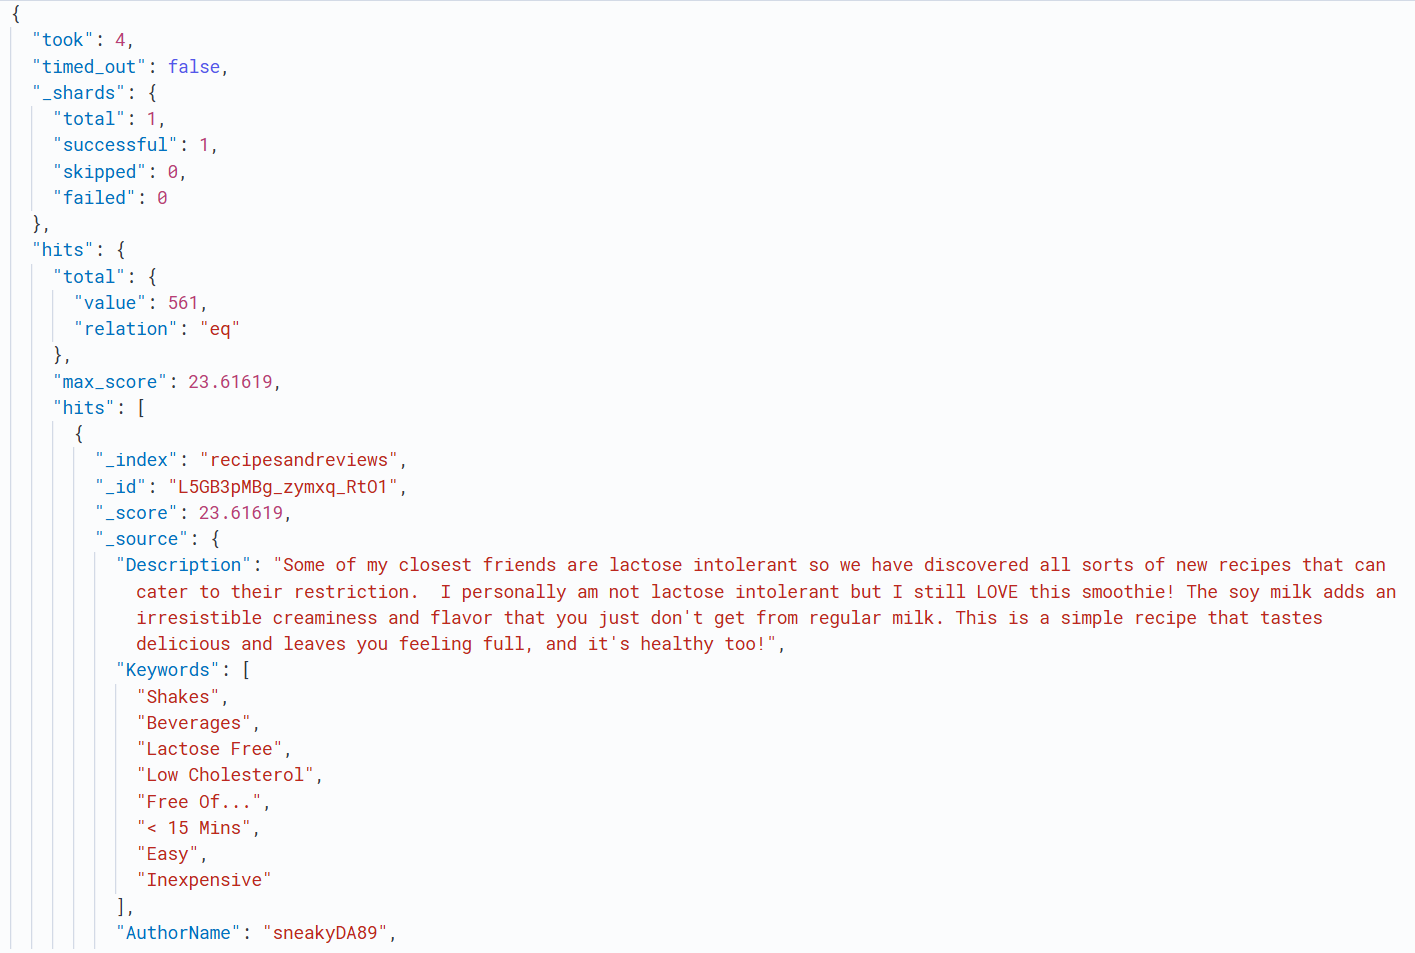
\includegraphics[width=0.9\linewidth]{Report/ReportLatex/Images/ElasticsearchResults/lactose1.png}
    \caption{1st result}
    \label{fig:enter-label}
    \end{figure}
    \begin{figure}[H]
    \centering
    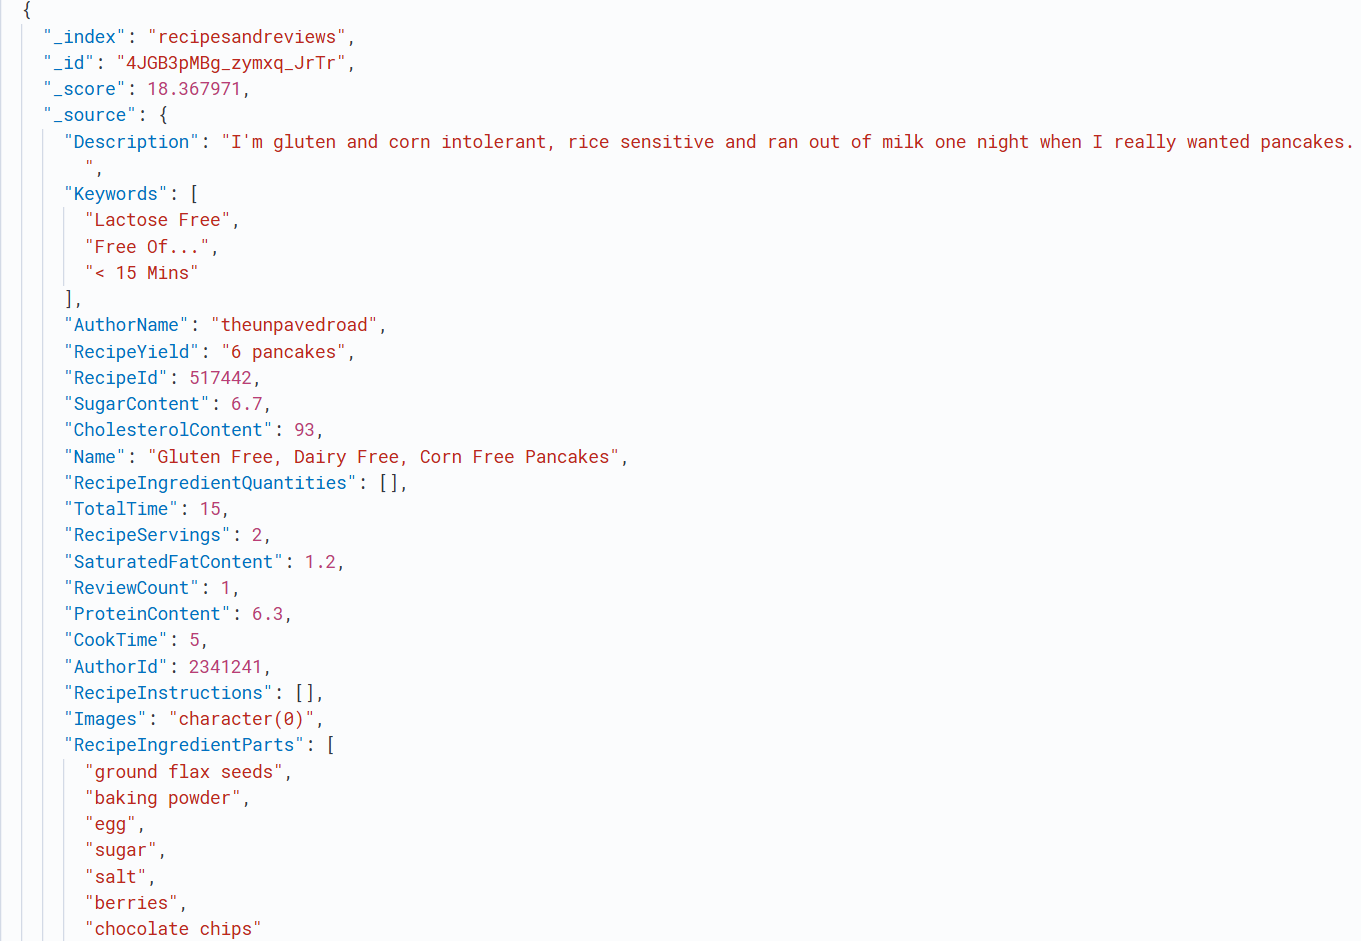
\includegraphics[width=0.9\linewidth]{Report/ReportLatex/Images/ElasticsearchResults/lactose2.png}
    \caption{2nd result}
    \label{fig:enter-label}
    \end{figure}
    \clearpage
    
    \item \addcontentsline{toc}{subsection}{Query 7 - Query to analyze the correlation between macronutrient ranges and calorie content}
          \textbf{Query to analyze the correlation between macronutrient ranges and calorie content}

    This Elasticsearch query is designed to analyze the relationship between calorie content and macronutrient distribution in recipes, aiming to uncover potential correlations. Recipes are grouped into predefined calorie ranges: low (under 1400 calories), medium (1400 to 2000 calories), and high (over 2000 calories). Within each calorie range, recipes are further categorized based on their levels of protein, fat, fiber, and sugar. Each nutrient is divided into three ranges: low, medium, and high, defined by thresholds such as grams of protein, fat, fiber, or sugar.

    The query uses a top-level aggregation to group recipes by calorie ranges. Nested within each calorie group, sub-aggregations further divide recipes into nutrient-specific ranges, such as low protein (less than 5g), medium protein (5–15g), or high protein (more than 15g). The focus is not on retrieving individual recipes but on generating summarized data that describes the nutritional characteristics within each calorie group.

    This approach allows for the examination of how macronutrient levels vary with calorie content, helping to identify trends or patterns.

    \subsubsection{Query}
    \begin{lstlisting}[language=Elasticsearch]
GET /recipesandreviews/_search
{
  "size": 0,
  "aggs": {
    "calorie_ranges": {
      "range": {
        "field": "Calories",
        "ranges": [
          { "to": 1400, "key": "Low calorie" },
          { "from": 1400, "to": 2000, "key": "Medium calorie" },
          { "from": 2000, "key": "High calorie" }
        ]},
      "aggs": {
        "protein_ranges": {
          "range": {
            "field": "ProteinContent",
            "ranges": [
              { "to": 5, "key": "Low protein" },
              { "from": 5, "to": 15, "key": "Medium protein" },
              { "from": 15, "key": "High protein" }
            ]}},
        "fat_ranges": {
          "range": {
            "field": "FatContent",
            "ranges": [
              { "to": 5, "key": "Low fat" },
              { "from": 5, "to": 15, "key": "Medium fat" },
              { "from": 15, "key": "High fat" }
            ]}},
        "fiber_ranges": {
          "range": {
            "field": "FiberContent",
            "ranges": [
              { "to": 1, "key": "Low fiber" },
              { "from": 1, "to": 5, "key": "Medium fiber" },
              { "from": 5, "key": "High fiber" }
            ]}},
        "sugar_ranges": {
          "range": {
            "field": "SugarContent",
            "ranges": [
              { "to": 5, "key": "Low sugar" },
              { "from": 5, "to": 15, "key": "Medium sugar" },
              { "from": 15, "key": "High sugar" }
            ]}}}}}}
    \end{lstlisting}

    \subsubsection{Result}
    The images display the output up to the end of the first bucket aggregation (low calorie).

    \begin{figure}[h!]
    \centering
    \begin{minipage}{0.25\textwidth}
        \centering
        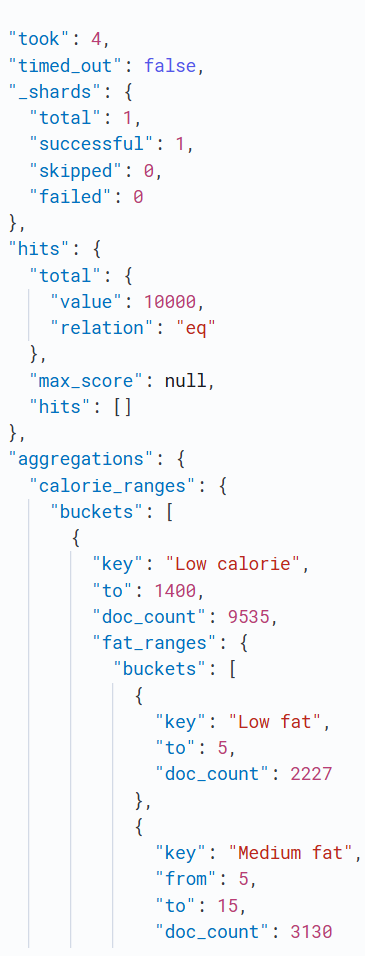
\includegraphics[width=\textwidth]{Report/ReportLatex/Images/ElasticsearchResults/calories1.png}
    \end{minipage}%
    \hspace{0.05\textwidth}
    \begin{minipage}{0.25\textwidth}
        \centering
        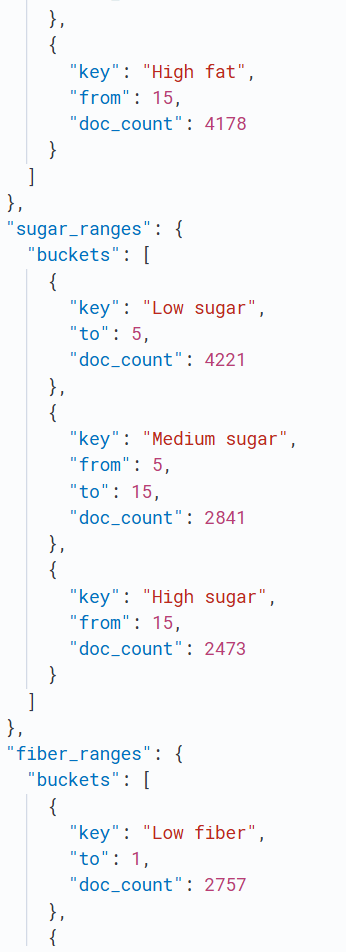
\includegraphics[width=\textwidth]{Report/ReportLatex/Images/ElasticsearchResults/calories2.png}
    \end{minipage}%
    \hspace{0.05\textwidth}
    \begin{minipage}{0.25\textwidth}
        \centering
        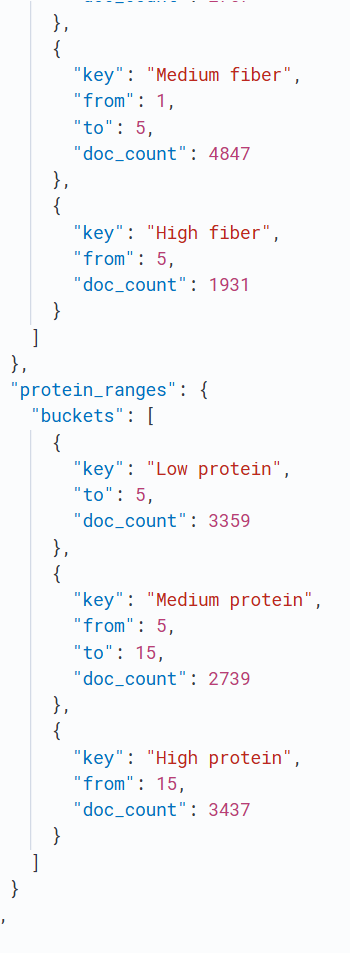
\includegraphics[width=\textwidth]{Report/ReportLatex/Images/ElasticsearchResults/calories3.png}
    \end{minipage}
    
    \caption{Output}
    \end{figure}
    
    \clearpage
    
    \item \addcontentsline{toc}{subsection}{Query 8 - Healthy, high-protein snacks that are not desserts}
          \textbf{Healthy, high-protein snacks that are not desserts}

    This query is designed to find snack recipes that are specifically healthy and high in protein, while excluding any recipes that fall under the dessert category. It starts by using the must clause to filter recipes that fall into the "Snacks" category and contain at least 20 grams of protein. These two conditions ensure that the results are relevant to the searcher's criteria for protein-packed snacks.

    In addition to these foundational requirements, the query includes a should clause to boost recipes that explicitly reference "healthy snack" in the description, reviews, or keywords. The use of the operator: "and" within the match queries means that the terms "healthy" and "snack" must both be present in these fields, increasing the likelihood of finding recipes that are truly aligned with the searcher's goal of a healthy, protein-rich snack.

    Furthermore, the query includes a must\_not clause to explicitly exclude recipes that are categorized as "dessert" or contain the term "dessert" in their keywords. This is important because the user wants to avoid any recipes that may be high in sugar or calories, which are often found in dessert items.

    \subsubsection{Query}
    \begin{lstlisting}[language=Elasticsearch]
GET /recipesandreviews/_search
{
  "query": {
    "bool": {
      "must":[
        {"match": {"RecipeCategory": "Snacks"}},
        {"range": { "ProteinContent": { "gte": 20 } } }
      ],
      "should": [
        { "match": { 
            "Description": {
              "query": "healthy snack",
              "operator": "and"
            } } },
        {
          "nested": {
            "path": "Reviews",
            "query": {
              "match": {
                "Reviews.Review": {
                  "query": "healthy snack",
                  "operator": "and"
                }}}}},
        {
          "match": {
            "Keywords": {
              "query": "healthy snack"
            }}}],
      "must_not": [
        { "match":{"RecipeCategory": "dessert"} },
        { "match":{"Keywords": "dessert"} }
      ]}}}
    \end{lstlisting}

    \subsubsection{Result}
    The images display the beginning of the first and second results, along with the preceding metadata.
    \begin{figure}[H]
    \centering
    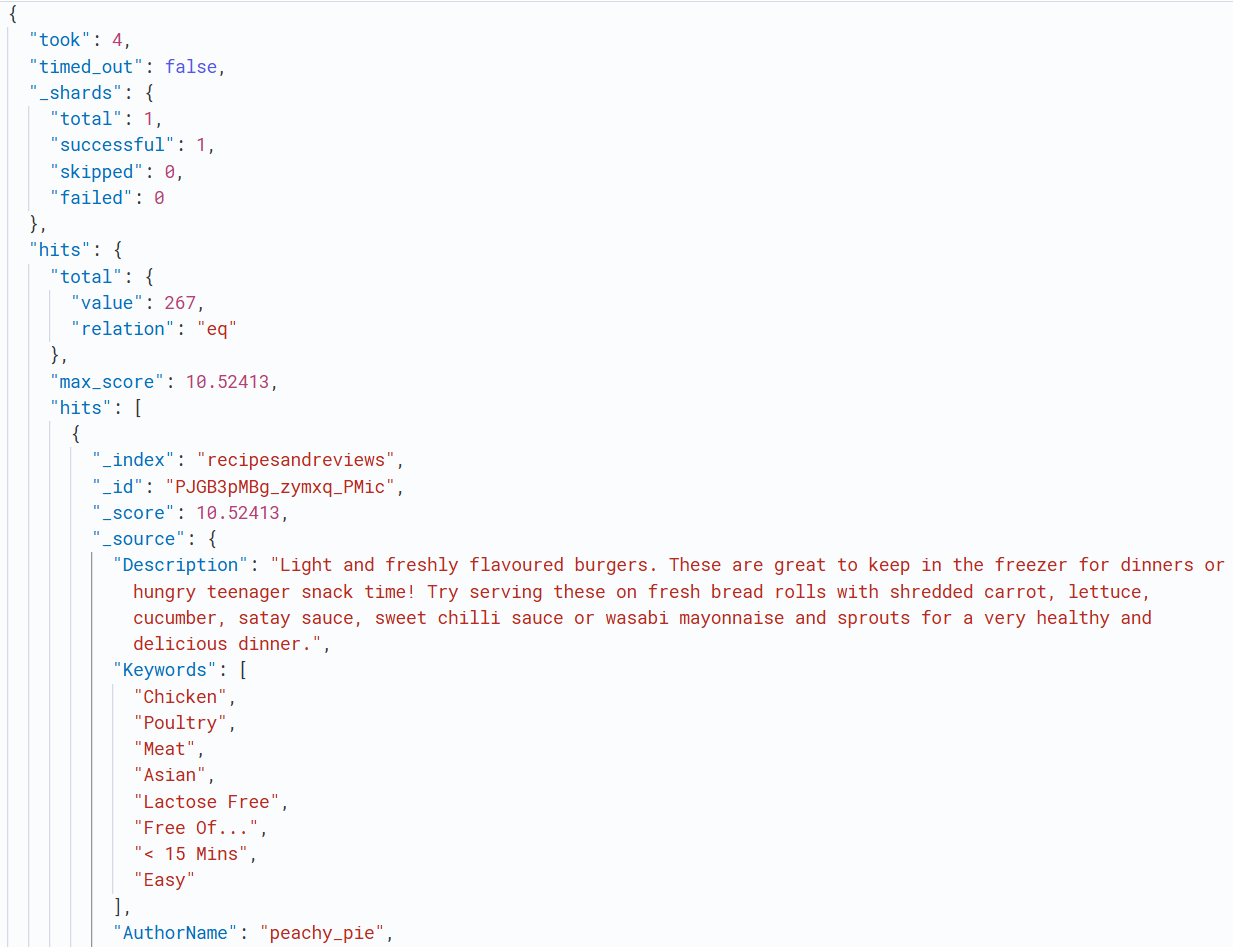
\includegraphics[width=0.8\linewidth]{Report/ReportLatex/Images/ElasticsearchResults/snack1.png}
    \caption{1st result}
    \label{fig:enter-label}
    \end{figure}
    \begin{figure}[H]
    \centering
    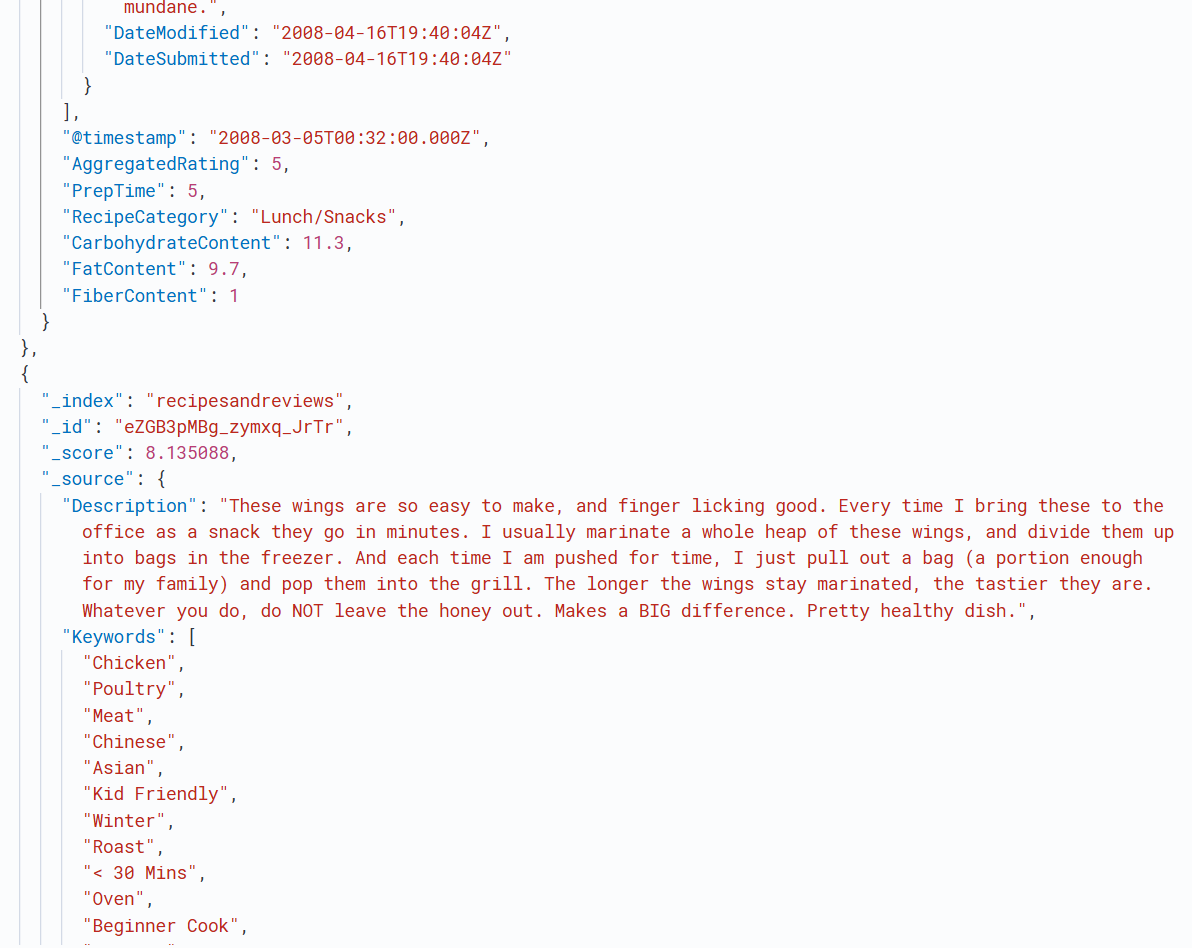
\includegraphics[width=0.8\linewidth]{Report/ReportLatex/Images/ElasticsearchResults/snack2.png}
    \caption{2nd result}
    \label{fig:enter-label}
    \end{figure}
    \clearpage
    
    \clearpage
    
    \item \addcontentsline{toc}{subsection}{Query 9 - Query that finds the authors with the best reviews}
          \textbf{Query that finds the authors with the best reviews}

    This query is designed for users who are looking to find accredited recipe authors to be inspired by, based on the quality of their recipes and the positive feedback they receive. By identifying authors with the best-reviewed recipes, this query helps users discover trustworthy sources for highly-rated dishes.

    The search starts with a must clause to ensure that only recipes with an AggregatedRating of 4 or higher are included, meaning the recipes are highly rated. Additionally, it filters out recipes with fewer than 10 reviews using a range query within the must clause on the ReviewCount field. This ensures that the results represent recipes that are well-reviewed by a significant number of people, giving a more reliable picture of the author's reputation.

    To further refine the results, the query includes a nested query within the Reviews field, looking for specific positive terms such as "great", "excellent", "good", "amazing" and "awesome." This helps identify recipes that have reviews with a positive sentiment. The operator: "or" in the query ensures that any of these positive words will contribute to the match, making it easier to capture a variety of positive sentiments across different reviews.

    The aggregation part of the query then groups the results by AuthorId using a terms aggregation, which enables the query to list authors who have the best reviews. Within each author group, the average\_rating aggregation computes the average AggregatedRating for their recipes. This provides a way to rank authors based on the quality of their work, specifically those who consistently receive high ratings.

    \subsubsection{Query}
    \begin{lstlisting}[language=Elasticsearch]
GET /recipesandreviews/_search
{
  "size": 1,
  "query": {
    "bool": {
      "must": [
        {"range": { "AggregatedRating": { "gte": 4} } },
        {"range": { "ReviewCount": { "gte": 10 } } },
        {"nested":{
          "path": "Reviews",
          "query": {
            "match": {
              "Reviews.Review": {
                "query": "great excellent good amazing awesome delicious yummy",
                "operator": "or"
            }}}}}]}},
  "aggs": {
    "positive_sentiment_per_author": {
      "terms": {
        "field": "AuthorId"
      },
      "aggs": {
        "average_rating": {
          "avg": {
            "field": "AggregatedRating"
          }}}}}}
    \end{lstlisting}

    \subsubsection{Result}
    The pictures below display the first document returned by the query and the beginning of the output section showing the aggregations.
    \begin{figure}[H]
    \centering
    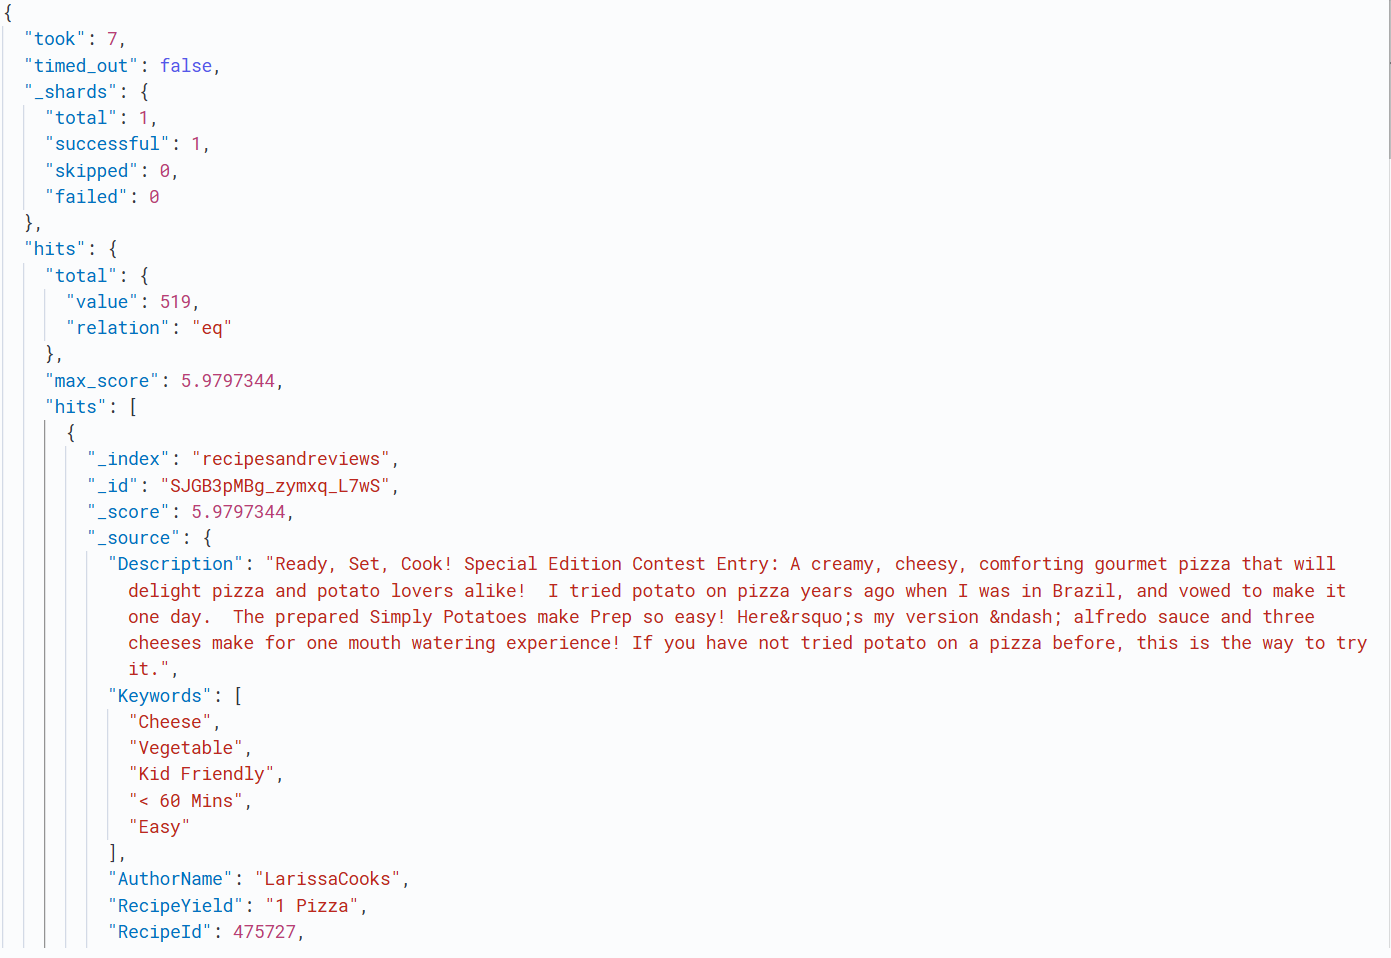
\includegraphics[width=0.8\linewidth]{Report/ReportLatex/Images/ElasticsearchResults/authors1.png}
    \caption{1st result}
    \label{fig:enter-label}
    \end{figure}
    \begin{figure}[H]
    \centering
    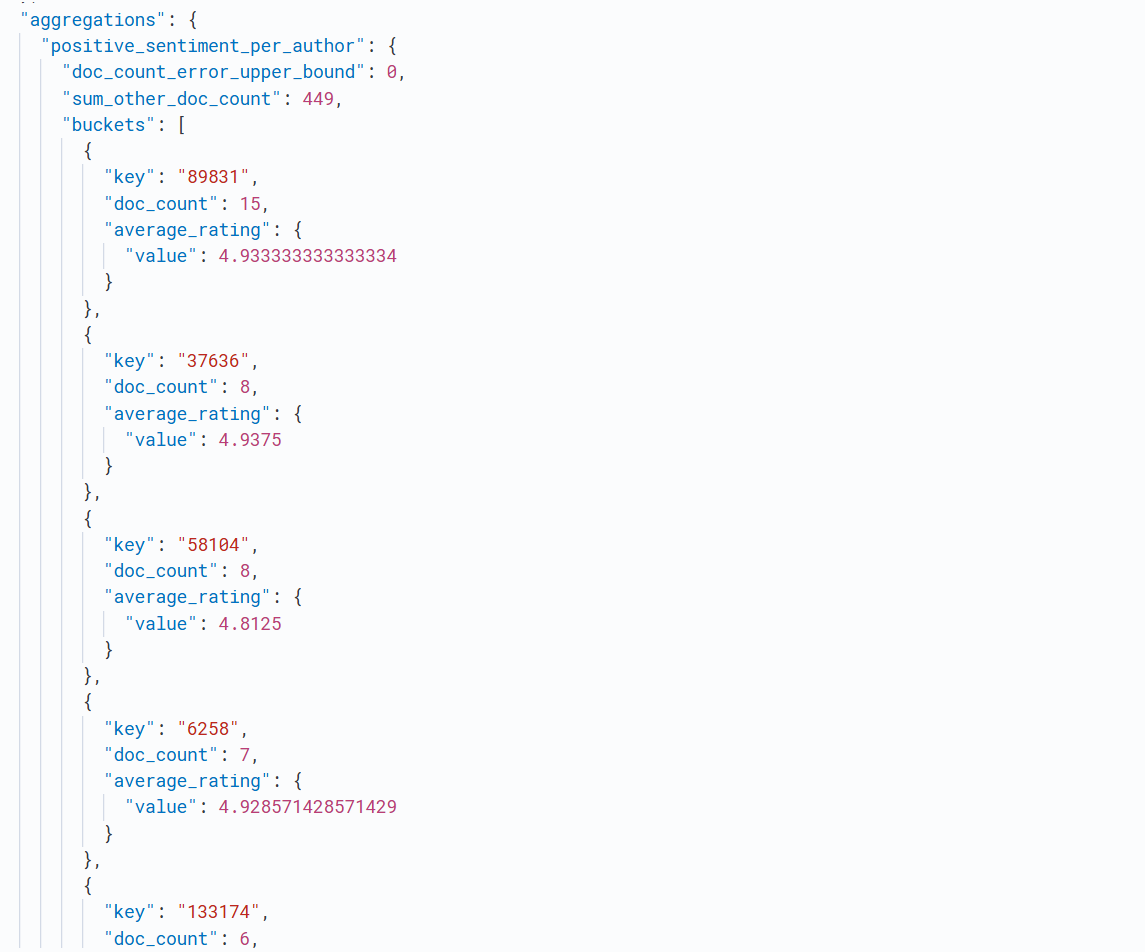
\includegraphics[width=0.8\linewidth]{Report/ReportLatex/Images/ElasticsearchResults/authors2.png}
    \caption{Aggregation output}
    \label{fig:enter-label}
    \end{figure}
    \clearpage
    
    \item \addcontentsline{toc}{subsection}{Query 10 - Easy, budget-friendly recipes ideal for students}
          \textbf{Easy, budget-friendly recipes ideal for students}

    This query is designed to find recipes that are ideal for college students looking for affordable and easy meal options. The query searches for recipes that are tagged with keywords or descriptions related to "college student" "cheap" and "easy". These terms are looked for in various fields such as the Description, Keywords, and RecipeCategory to ensure that the results are tailored to the needs of students who are on a budget and looking for simple meal ideas. Additionally, the query looks within Reviews to capture any references to these themes, which helps in identifying recipes that other students have positively reviewed for being cost-effective and easy to prepare.

    To ensure the recipes are practical for busy students, the query includes a must\_not clause that filters out recipes requiring more than 60 minutes of total time. This ensures that only quick and efficient recipes are returned, as students often do not have the luxury of long cooking times. The use of the minimum\_should\_match parameter ensures that the query returns recipes that meet at least one of the keyword or descriptive criteria, providing a diverse set of relevant results.

    \subsubsection{Query}
    \begin{lstlisting}[language=Elasticsearch]
GET /recipesandreviews/_search
{
  "query": {
    "bool": {
      "should": [
          {"match":
            {
              "Description": {
                "query": "college student cheap easy",
                "operator": "or"
              }}},
          {"match":
            {
              "Keywords": {
                "query": " college student cheap easy",
                "operator": "or"
              }}},
          {"match":
            {
              "RecipeCategory": {
                "query": "college student cheap easy",
                "operator": "or"
              }}},
          {"nested":{
          "path": "Reviews",
          "query": {
            "match": {
              "Reviews.Review": {
                "query": "college student cheap easy",
                "operator": "or"
            }}}}}],
      "must_not": [
        {
          "range": {
            "TotalTime": {
              "gte": 60
            }}}],
      "minimum_should_match": 1
    }}}
    \end{lstlisting}

    \subsubsection{Result}
    The pictures below display the first document returned by the query.
    \begin{figure}[H]
    \centering
    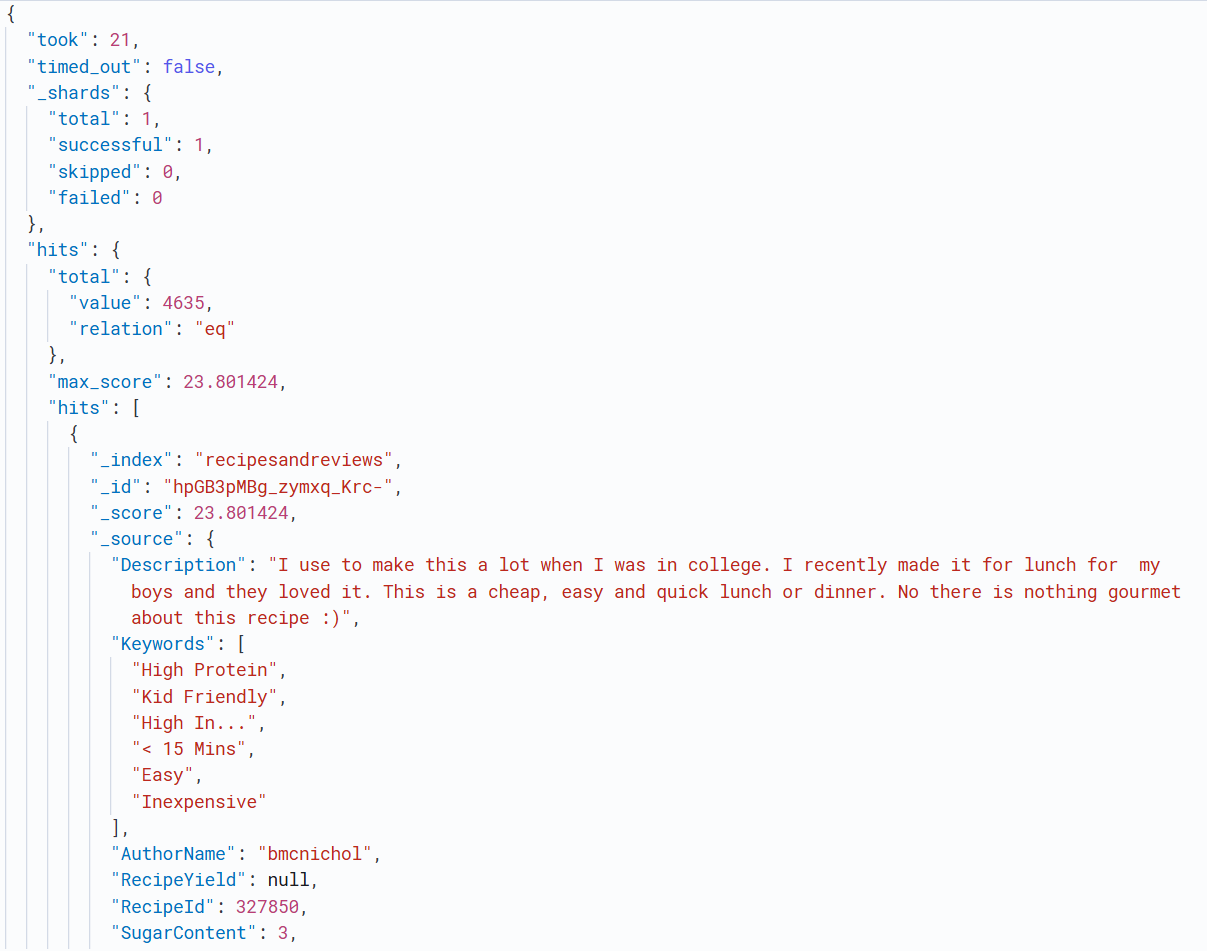
\includegraphics[width=0.7\linewidth]{Report/ReportLatex/Images/ElasticsearchResults/college1.png}
    \caption{1st result (pt.1)}
    \label{fig:enter-label}
    \end{figure}
    \begin{figure}[H]
    \centering
    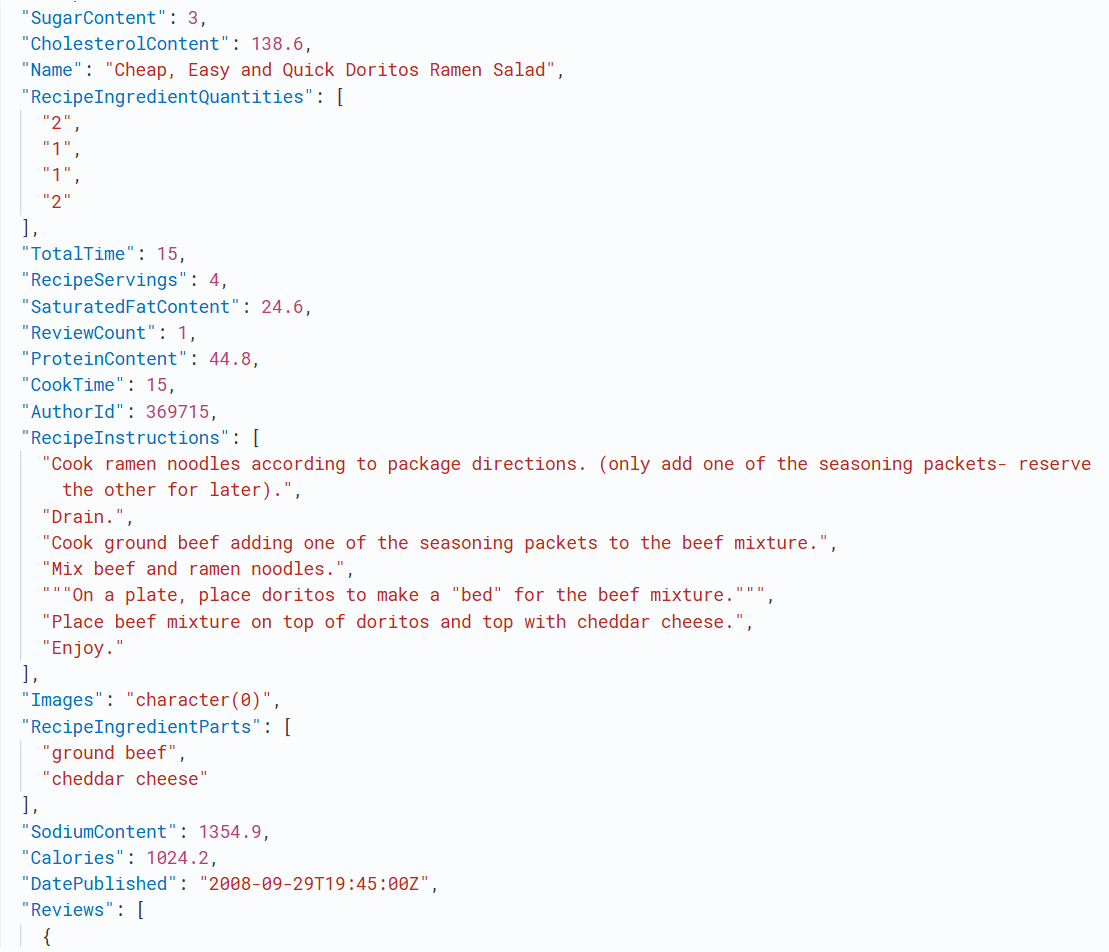
\includegraphics[width=0.7\linewidth]{Report/ReportLatex/Images/ElasticsearchResults/college2.png}
    \caption{1st result (pt.2)}
    \label{fig:enter-label}
    \end{figure}
    \begin{figure}[H]
    \centering
    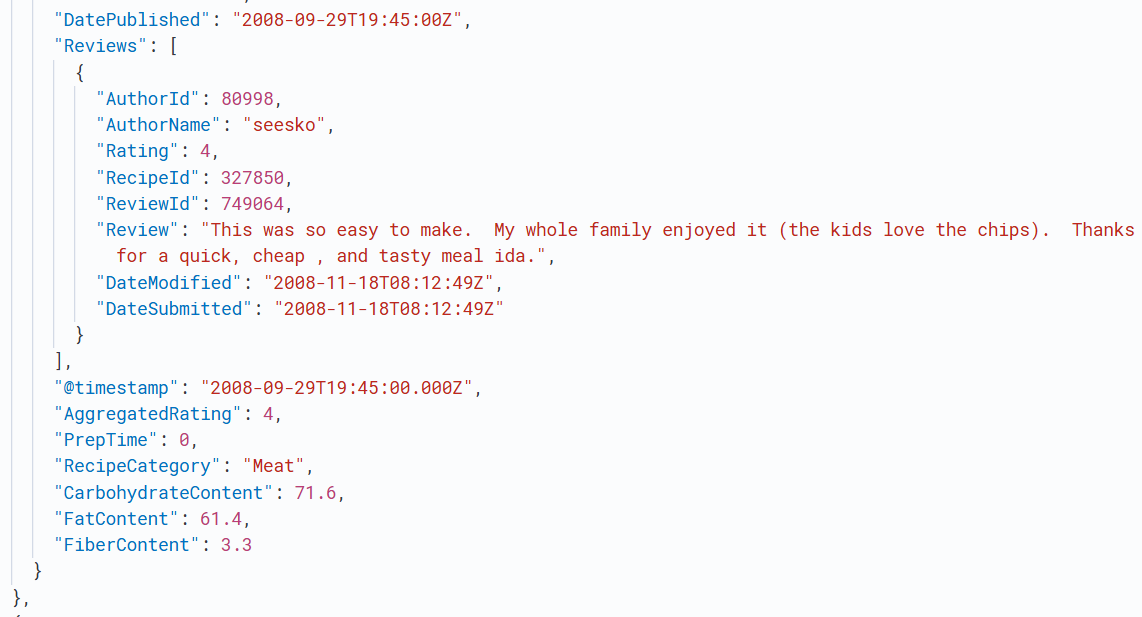
\includegraphics[width=1\linewidth]{Report/ReportLatex/Images/ElasticsearchResults/college3.png}
    \caption{1st result (pt.3)}
    \label{fig:enter-label}
    \end{figure}
\end{enumerate}
\chapter{Extra}
\section{Taste trios - the web app}
In order to put this project's results to use in a "production environment" a small web app have been developed. Due to time, knowledge, and resource constraints, the developed system is meant to be more of a proof of concept than an actual finished product.

The latest release of the "Taste Trios" application can be found \textbf{\href{https://taste-trios-front-end.vercel.app/}{here}}

\subsection{Goals and principles$\implies$Feature selection}
In order to guide the development process the following goals/principles have been identified:
\begin{itemize}
    \item The system must be fully deployed and accessible from anywhere
    \item The total monetary cost of keeping the system running must amount to no more than \EUR{0}
    \item Embracing the "proof of concept" mentality the system is not meant to handle a large user base and the overall performance is not a major concern
    \item "Functionality over aesthetics" (a must given the authors' background)
    \item The system must provide useful features for the targets of the analysis: off-site students
    \item The system must interact with both the chosen NoSQL technologies (Neo4J, ElasticSearch) in a meaningful way
\end{itemize}

Given those guidelines, the following features have been chosen:
\begin{enumerate}
    \item \textbf{Pan-try it out}: A page that, given a list of ingredients, finds recipes that utilize the biggest number of them. This feature can be useful when trying to finish food supplies before the Winter break.
    \item \textbf{Mix \& Max}: A page that, given a list of ingredients, finds which ingredients "pairs" the best with the given ones. The page can also suggest recipes with the matched ingredients. This feature can be helpful when deciding what to buy while grocery shopping.
    \item \textbf{Elasticsearch Queries}: Reading JSONs can be daunting. This motivates the development of a page where both the presented Elasticsearch queries and their respective results are interpreted and made readable.
\end{enumerate}

\subsection{System Architecture and Design choices}
The system is designed with a \textbf{three-tier architecture}, consisting of the \textbf{Presentation Layer (Front End)}, \textbf{Logic Layer (Backend)}, and \textbf{Data Layer}. Each layer utilizes modern (and free to use) technologies and deployment platforms to ensure efficiency, scalability, and maintainability.

\subsubsection{Presentation Layer (Front End)}

\begin{itemize}
\item \textbf{Technology Stack}: React and Next.js
\item \textbf{Deployment}: \href{https://vercel.com/}{Vercel}
\item \textbf{Role}:
\begin{itemize}
\item Provides an interactive user interface (UI).
\item Handles client-side routing and server-side rendering using Next.js.
\item Ensures seamless user interaction by dynamically updating the UI without requiring full-page reloads.
\end{itemize}
\item \textbf{Communication}:
\begin{itemize}
\item Utilizes HTTPS protocols to communicate with the backend.
\item Exchanges data in JSON format via RESTful APIs.
\end{itemize}
\end{itemize}

\subsubsection{Logic Layer (Backend)}

\begin{itemize}
\item \textbf{Technology Stack}: Flask (a Python-based microframework)
\item \textbf{Deployment}: \href{https://vercel.com/}{Vercel}
\item \textbf{Role}:
\begin{itemize}
\item Manages requests from the front end and formulates responses by interacting with the Data Layer.
\end{itemize}
\item \textbf{Communication}:
\begin{itemize}
\item Exposes RESTful APIs over HTTPS.
\item Exchanges data with the front end in JSON format.
\end{itemize}
\end{itemize}

\subsubsection{Data Layer}

The Data Layer is composed of two databases that are set up and filled as described previously:

\subsubsection{Neo4j}
\begin{itemize}
\item \textbf{Hosting}: \href{https://neo4j.com/product/auradb/}{AuraDB(free tier)}
\item \textbf{Role}:
\begin{itemize}
\item Manages data represented as nodes and relationships, enabling complex queries and graph-based analytics.
\item Ideal for use cases like relationship mapping and network analysis.
\end{itemize}
\item \textbf{Communication}:
\begin{itemize}
\item Interacts with the Logic Layer via REST APIs.
\item Queries are written in Cypher.
\end{itemize}
\end{itemize}

\subsubsection{Elasticsearch}
\begin{itemize}
\item \textbf{Hosting}: \href{https://bonsai.io/}{Bonsai(free tier)}
\item \textbf{Role}:
\begin{itemize}
\item Facilitates fast and efficient text-based searches and analytics.
\item Handles indexing, filtering, and ranking of large datasets.
\end{itemize}
\item \textbf{Communication}:
\begin{itemize}
\item Interacts with the Logic Layer via Elasticsearch's RESTful API.
\item Exchanges data in JSON format.
\end{itemize}
\end{itemize}

\subsubsection{Serverless Aspects of the Architecture}
\href{https://vercel.com/}{Vercel} is a serverless platform, meaning there is no need to manage or provision servers for deploying and running both the React/Next.js application and the Python backend. Static assets and server-side rendered pages are served dynamically, scaling automatically based on traffic.
The serverless paradigm has been chosen for the following benefits:
\begin{itemize}
\item Automatic scaling.
\item Simplified deployment and infrastructure maintenance.
\end{itemize}

\subsection{Backend APIs}
To achieve the desired servers, the following backend API endpoints have been developed:

\begin{itemize}
\item\hypertarget{fun:checkIngredient} {\textbf{/api/neo4j/checkIngredient (POST)}}: Checks if a specified ingredient exists in the database. The request body contains the ingredient name. Since the ingredients are used both in Neo4J and ElasticSearch queries, an exact match is needed, thus this check the existence of the ingredient in the stricter DB: Neo4j. The following query is performed:
\begin{CypherQuery}
.
MATCH (n:Ingredient) WHERE n.name = \$ingredient RETURN n
\end{CypherQuery}

\item \textbf{/api/neo4j/matchIngredients (POST)}: Matches recipes containing at least one of the provided ingredients. Returns recipes sorted by the number of matching ingredients. The request body contains the ingredient name and a limit on the number of responses.
The following query is performed:
\begin{CypherQuery}
.
MATCH (r:Recipe)-[:CONTAINS]->(i:Ingredient)
WHERE i.name IN \$ingredients
WITH r, count(i) AS matchingScore, COLLECT(i.name) AS matchingIngredients
RETURN r, matchingScore, matchingIngredients ORDER BY matchingScore DESC
LIMIT \$limit
\end{CypherQuery}

\item \hypertarget{fun:elasticsearch/matchIngredients}{\textbf{/api/elasticsearch/matchIngredients (POST)}}: Performs a similar function as above but uses Elasticsearch to query indexed recipe data. This allows fuzzier matches that can be desirable when dealing with user inputs.
The following query is performed:
\begin{lstlisting}[language=Elasticsearch]
{
    "query": {
        "bool": {
            "should": [{
                "match": {
                    "RecipeIngredientParts": {
                        "query": " ".join(ingredients),
                        "operator": "or"
                    }
                }
            }]
        }
    }
}
\end{lstlisting}

\item \hypertarget{fun:matchIngredientsAnd}{\textbf{/api/elasticsearch/matchIngredientsAnd (POST)}}: Returns recipes containing a specifically required ingredient and at least one additional ingredient from a provided list. The request body contains the ingredient list whose last item is the one that must be matched and a limit on the number of responses. The following query is performed:
\begin{lstlisting}[language=Elasticsearch]
{
    "query": {
        "bool": {
            "filter": [
                {
                    "match":{
                         "RecipeIngredientParts": ingredients[-1]
                     }
                 }
            ],
            "must": [
                {
                    "match": {
                        "RecipeIngredientParts": {
                            "query": " ".join(ingredients[:-1]),
                            "operator": "or"
                        }
                    }
                }
            ]
        }
    }
}
\end{lstlisting}

\item \textbf{/api/neo4j/getIngredients (POST)}: Retrieves all ingredients necessary for a specified recipe. The request body contains the id of the recipes. The following query is performed:
\begin{CypherQuery}
.
MATCH (r:Recipe)-[:CONTAINS]->(i:Ingredient)
WHERE r.id = \$recipe
RETURN COLLECT(i.name) AS ingredients
\end{CypherQuery}

\item \hypertarget{fun:mixAndMax}{\textbf{/api/neo4j/mixAndMax (POST)}}: Suggests additional ingredients that maximize recipe compatibility based on the provided ingredients. The following query is performed: 
\begin{CypherQuery}
.
WITH \$providedIngredients AS ingredients
// Find recipes that contain an existing ingredient and additional matched ingredients
MATCH (i:Ingredient)<-[:CONTAINS]-(r:Recipe)-[:CONTAINS]->(i1:Ingredient)
WHERE i.name IN ingredients AND NOT i1.name IN ingredients
WITH DISTINCT r, i1.name AS matchedIngredient, ingredients, COUNT(distinct i) as availableMatchedIngredients

// Match reviews for these recipes and calculate the average rating for each matched recipe
MATCH (r)<-[:FOR]-(rev:Review)
WITH matchedIngredient, r, AVG(rev.rating) AS avgRating, ingredients, availableMatchedIngredients

// Count the number of unique recipes for each matched ingredient
MATCH (r)-[:CONTAINS]->(i:Ingredient)
WHERE i.name IN ingredients
RETURN matchedIngredient, COUNT(DISTINCT r) AS recipeCount, AVG(avgRating) AS avgOfAvgRatings, AVG(availableMatchedIngredients) as IngredientCompatibility
ORDER BY IngredientCompatibility * log10(recipeCount) DESC
\end{CypherQuery}
\item \hypertarget{elasticsearch/queries}{\textbf{/api/elasticsearch/queries (GET)}}: Runs predefined Elasticsearch queries based on a query number parameter. The performed queries are the one described in Section \ref{sec:ElastisearchQueries}
\end{itemize}

\subsection{Feature implementation}
\subsection*{Pan-try it out}
This feature has been implemented as follows:
\newcommand{\hyperLinkToAPI}[1]{\hyperlink{fun:#1}{\textbf{#1}}}
\begin{enumerate}
    \item The user can insert the desired ingredients in the input bar.
    \item Upon submission the inserted ingredient is validated using \hyperLinkToAPI{checkIngredient}
    \item Upon validation, recipe suggestions are obtained through \hyperLinkToAPI{elasticsearch/matchIngredients}
    \item The matched recipes are displayed and the distribution of various attributes of the matched recipes are computed and plotted
\end{enumerate}

\subsection*{Mix \& Max}
This feature has been implemented as follows:

\begin{enumerate}
    \item The user can insert the desired ingredients in the input bar.
    \item Upon submission the inserted ingredient is validated using \hyperLinkToAPI{matchIngredientsAnd}
    \item Upon validation, ingredient suggestions are obtained by calling  \hyperLinkToAPI{mixAndMax}
    \item The matched ingredients are displayed and the distribution of various attributes of the matched recipes are computed and plotted
    \item If the user presses on an ingredient, recipe suggestions are obtained using \hyperLinkToAPI{matchIngredientsAnd}, passing the selected ingredient as the last one,
    and are displayed in a modal.
\end{enumerate}

\subsection*{Elasticsearch queries}
This feature has been implemented as follows:

\begin{enumerate}
    \item The user can select one of the ten queries.
    \item The selected query's body is displayed as a tree structure using a custom-made JSON parser
    \item The user can then decide to run the query by pressing the appropriate button, which in turn calls \hyperLinkToAPI{elasticsearch/queries} with the right query number
    \item The result of the query is then displayed. The majority of the queries return a set of recipes that are displayed as in the other features. Two of them return some aggregations that are displayed using the JSON tree parser
\end{enumerate}

\cleardoublepage
% LIST OF FIGURES
\listoffigures

% LIST OF TABLES
\listoftables

\cleardoublepage

\end{document}
